\documentclass[a4paper,11pt]{article}
%%%%%%%%%%%%%%%%%%
%%%%%%%%%%%%%%%%%
%% NON USARE MACRO CON MATH perché 4ht NON converte correttamente!
%% $\mathup{qR}_3^*$ deve essere scritto direttamente!
%%%%%%%%%%%%%%%%%
\usepackage{lib/common_definitions}
%###
\begin{document}
\title{CSTN Benchmarks}
\author{Roberto Posenato\\
	Dipartimento di Informatica\\
	Università degli Studi di Verona, Italy}
\date{2018-02-21}

\ifpdf
\maketitle
\fi 

\section{Introduction}
\blankfootnote{The original version of this document can be download at \url{http://profs.scienze.univr.it/~posenato/software/cstnu/tex/benchmarks.pdf}}

During the research about temporal networks, we prepared some benchmarks for testing some algorithms:
\begin{itemize}
\item  \href{http://profs.scienze.univr.it/~posenato/software/benchmarks/CSTNBenchmark2016.tgz}{CSTNBenchmark2016} and \href{http://profs.scienze.univr.it/~posenato/software/benchmarks/CSTNBenchmark2018.tgz}{CSTNBenchmark2018}: for testing Dynamic Consistency (DC) checking algorithms for Conditional Simple Temporal Networks (CSTNs).

\item  \href{http://profs.scienze.univr.it/~posenato/software/benchmarks/CSTNUBenchmark2018.tgz}{CSTNUBenchmark2018}: for testing Dynamic Controllability (DC) checking algorithms for Conditional Simple Temporal Networks with Uncertainty (CSTNUs).

\item \href{https://profs.scienze.univr.it/~posenato/software/benchmarks/STNUBenchmark2020.tgz}{STNUBenchmark2020}: for testing DC checking algorithms for Simple Temporal Networks with Uncertainty (STNUs).
\end{itemize} 

CSTNBenchmark2016 and CSTNBenchmark2018 benchmarks contain CSTN instances, CSTNUBenchmark2018 contains CSTNU instances while STNUBenchmark2020 contains STNU instances.

Some instances were determined transforming random workflows generated by the ATAPI Toolset~\cite{LanzR14}, while others (STNUs for example) were determined using ad-hoc random generator present in the CSTN Tool library.


\subsection{Temporal Networks From Random Workflows}
We considered a random workflow generator as source of random CSTN(U) instances for having a closer approximation to real-world instances and also for generating networks that are more difficult to check than those created haphazardly.

The ATAPI toolset produces random workflows according to different input parameters that govern the number of tasks, the probability of having parallel (AND)\slash alternative (XOR) branches, the probability of inter-task temporal constraints, and so on.
In particular, the ATAPIS toolset builds a workflow instance in two phases. In the first phase, it prepares the structure of the network in a recursive way starting from a pool of $N$ blocks representing tasks.
At each cycle, randomly it removes two blocks from the pool and casually decides how to combine them using an AND/XOR/SEQUENTIAL connector.
The resulting block is then added to the pool. The generation phase ends when there is only one block in the pool. 
The probability to choose an AND or an XOR connector can be given as input ($P_A$, and $P_C$ parameters).
Temporal constraints are added in the second phase considering some parameters that can be given as input. 
The following parameter-values were determined after some experiments where we tried to discover a good mix of them to  guarantee not trivial consistent\slash not consistent instances.
The chosen values were:
\begin{itemize}
\item each task duration is a subrange of $[2, 30]$; each bound is chosen according to a beta distribution;
\item each connector duration has always range $[1, 10]$;
\item each delay between sequential tasks is a subrange of $[1, 25]$; each bound is according to a beta distribution;
\item each delay between a connector and a task is fixed to $[1, 100]$;
\item the probability to have an inter-activity temporal constraint between any pair of activities (i.e, tasks or connectors) was set to $0.2$.
	In case that an inter-activity temporal constraint is set, its range is a casual subrange of the $[min distance, max distance]$ between the two activities, where min and max distances were calculated by the tool.
\end{itemize}

For generating CSTN instances, the method consisted in two phases:
\begin{itemize}
\item Fixed the above parameters, workflow graphs were randomly generated by varying the number of tasks ($N$), the probability for parallel branches ($P_A$), and the probability for alternative branches ($P_C$) to determine different blocks of instances; 
\item each workflow graph was then translated into an equivalent CSTN using the method proposed in~\cite{CombiGMP14}. Task durations were represented as ordinary constraints in CSTN instances.
\end{itemize}

For generating the CSTNU instances, the method used was similar to the above one for CSTN benchmarks. The only difference was that all task durations were translated as contingent links in corresponding CSTNU instances.

\subsection{Temporal Networks From a Random Generator}\label{SECT:STNUGenerator}
During the study of DC checking algorithm for STNU, we wanted to test the different polynomial-time algorithms using instances having significant size, i.e., a size much larger than the size of instances obtained in previous benchmarks for CSTN or CSTNU.
We verified that increasing the size of random workflow instances built using ATAPI toolset to have bigger STNU instances did not work because, for the characteristics of generated workflows, the obtained instances were almost not DC and the generation of few DC instances required a lot of computation.

Therefore, we decided to build a specific STNU random generator (\href{http://profs.scienze.univr.it/~posenato/software/cstnu/apidocs/it/univr/di/cstnu/algorithms/STNURandomGenerator.html}{it.univr.di.cstnu.algorithms.STNURandomGenerator}) capable of building big-size STNU instances.
Our STNU generator can build random instances having a chosen topology that can be tuned by a variety of input parameters.
The possible topologies are \textit{1) no-topology, 2) tree}, or \textit{3) worker-lanes}.
After some testing, we verified that the \textit{worker-lanes} topology, which simulates the worker-lanes of business process modeling~\cite{bpmi}, is the most interesting because it allows the generation of big random instances where there could be circuits involving many constraints. 
In this topology, the set of contingent links is partitioned into a given  number of lanes.
Contingent links within each lane are interspersed with ordinary constraints that
specify delays between the end of one contingent link and the start of the next.
Finally, there are constraints between pairs of nodes belonging to different lanes to represent temporal-coordination constraints among time-points. Typically, such constraints involve 
nodes on different lanes that are at a similar distance from the start of their respective lanes. 

As an example, Figure 1 depicts a portion of a random STNU having 500 nodes and 50 contingent links in a 5-worker-lane topology.
%\begin{figure}[tb]
\begin{center}
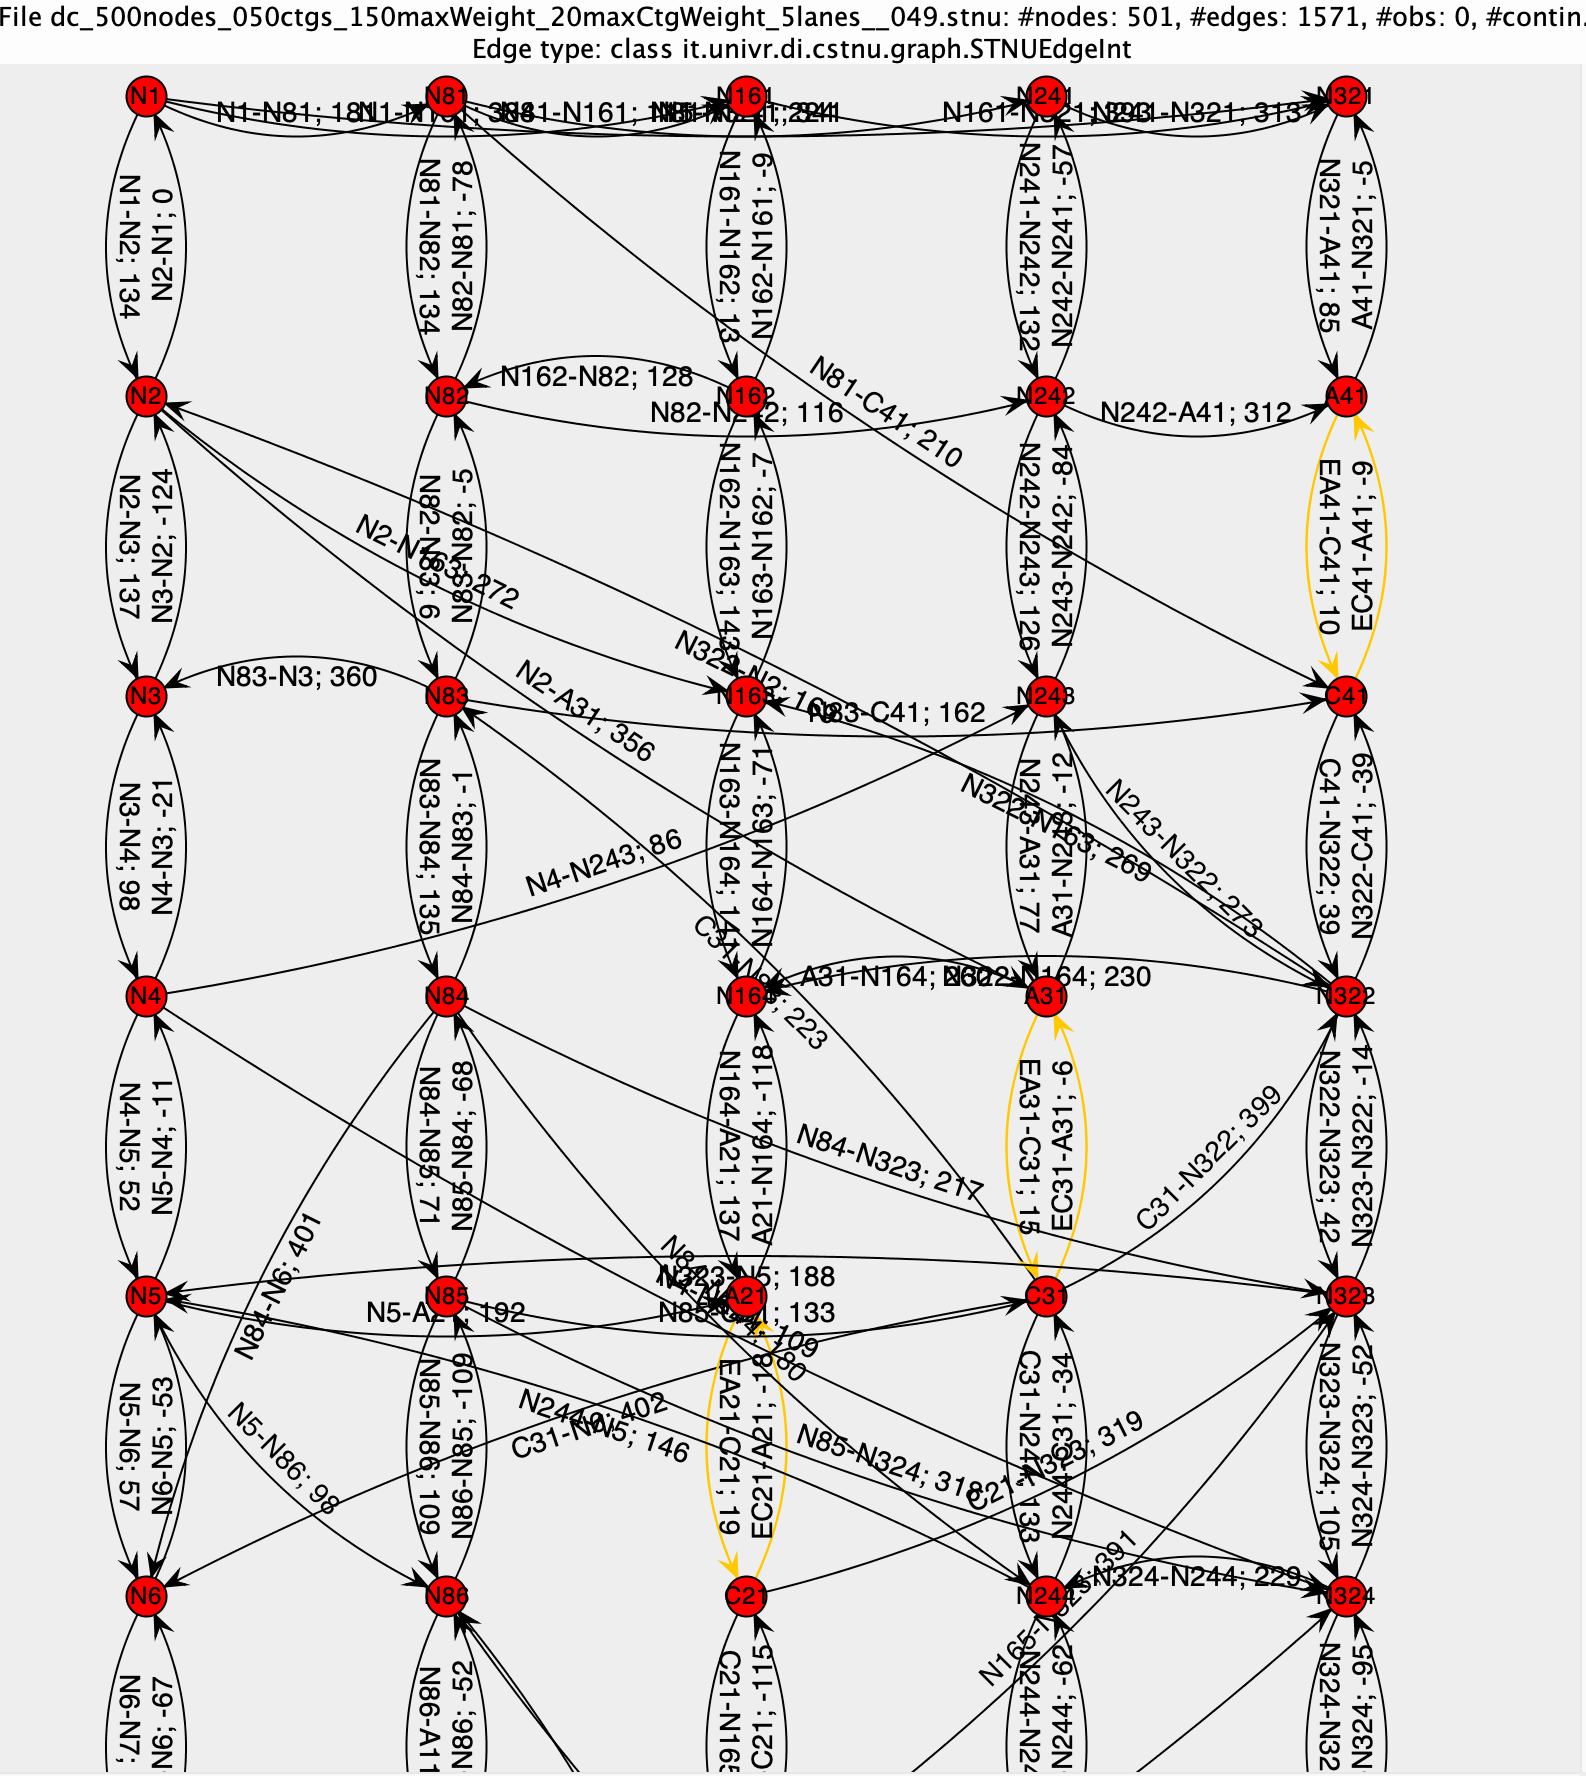
\includegraphics[angle=-90,width=.85\textwidth,keepaspectratio]{workerLaneSTNU}\\%height=.6\textheight
\textbf{Figure 1: An example of a randomly generated STNU}%\label{FIG:workerLaneSTNU}		
\end{center}
%\end{figure}

Many aspects of the worker-lanes topology can be tuned as input parameters;  
the number of nodes, the number of contingent links, the number of lanes, the probability of a temporal constraint for a pair of nodes from different lanes, the maximum weight of each contingent link, the maximum weight of each ordinary constraint, and so on.



\section{Benchmarks}
\subsection{CSTNBenchmark2016}

This benchmark is composed of four sub-benchmarks (named as \textit{benchmarks} in papers~\cite{time2015,HunsbergerP16Icaps,CairoEtalTime2017,HunsbergerPFixed18,HunsbergerPEpsilon18,HunsbergerP20}).
Each sub-benchmark is composed of two sets: one set of DC CSTN instances and one set of NOT DC ones.

Each sub-benchmark, characterized by a number $N$, is called  \textbf{Size$N$} and contains CSTN instances (DC\slash NOT DC) generated by random workflows having $N$ tasks, $k$ XOR connectors (= propositions in CSTN) and a variable number of AND connectors. 
The probability for parallel branches $P_A$ was fixed to 0.2 as well as the probability for alternative branches $P_C$. 

The following table summarizes the main characteristics of all sub-benchmarks:
\begin{center}
\begin{tabular}{rrrrr}
	\hline
  \textbf{benchmark}: & \textbf{size10}	& \textbf{size20}	& \textbf{size30}	& \textbf{size40}\\
  \hline
  \#tasks: & 10 & 20 & 30 & 40 \\ 
  $k$=\#XOR: & 3 & 5 & 7 & 9\\% & \rule{0in}{0.2in}
  \#CSTN-nodes: & 45-59 &79-95& 123-135&159-175\\
  \hline
\end{tabular}
\end{center}
For each sub-benchmark, there are at least 60 dynamically consistent CSTNs and 20 non-dynamically consistent CSTNs.
Since the original ATAPIS toolset allows one to fix only the probability of AND\slash XOR connectors, it was necessary to run the toolset a huge number of times for obtaining the instances with the above characteristics.

\smallskip
Different workflow graphs with the same number of tasks may translate into CSTNs of different sizes due to different numbers of AND connectors in the workflows.
This fact represented the main weakness of this benchmark. 
For example, even if for $N=10$ and $k=3$ there are 60 DC instances, such instances are CSTN instances with different order (=\#nodes). Few of them have the same order and this fact  represents a limitation when an evaluation of DC execution time with respect of the CSTN order is required. 

For this benchmark we do not report here the results obtained using our algorithms because they are superseded by the results obtained with CSTNBenchmark2018, presented in the next section.


\subsection{CSTNBenchmark2018}

The structure of this benchmark is equals to the CSTNBenchmark2016 benchmark one: four sub-benchmarks with two sets for each. 
The main differences are the number of instances and the structure of the instances.

After an important modification of ATAPI Toolset source code, it was possible to give as input also the number of XOR\slash AND connectors that a random workflow instance must have.
Therefore, it was possible to build sets of more uniform instances where the randomness could decide how to mix components and constraints but not their quantities.
It is possible to show that the relation between workflow component quantities and CSTN order is $5+2N+6k+4j$, where $N$ is the number of tasks, $k$ the number of XOR connectors, and $j$ the number of AND connectors. 
Therefore, for each possible planned combinatios of \#task-\#XOR-\#AND, it was possible to generate randomly 50 DC and 50 NOT DC instances.
The following table summarizes the characteristics of each sub-benchmark.
 \begin{center}
\begin{tabular}{@{} l >{\RaggedLeft\arraybackslash}p{1.4cm} >{\RaggedLeft\arraybackslash}p{1.5cm} >{\RaggedLeft\arraybackslash}p{1.5cm} >{\RaggedLeft\arraybackslash}p{1.3cm} c >{\RaggedLeft\arraybackslash}p{1.2cm} @{}}
	\hline
  \textbf{Group} &\textbf{Bench mark}  & \textbf{instance indexes} & \textbf{\# activities} & \textbf{\#XOR}	& \textbf{\#AND}	& \textbf{CSTN order}\\
  \hline		  
	Size010-3		& B10-3-0	&	000-049					&	10				&      3				&      0 		&	43\\	
				    & B10-3-1	&	050-099					&		10				&	  3				&	  1			&	47\\
					& B10-3-2	&	100-149					&		10				&		3		&		2		& 	51\\
					& B10-3-3	&	150-199					&		10				&		3		&		3		& 	55\\
					& B10-3-4	&	200-249					&		10				&		3		&		4		& 	59\\
	\hline					
	Size020-5		& B20-5-0	&	000-029					&		20				&		5		&		0		& 	75\\
					& B20-5-1	&	030-059					&		20				&		5		&		1		&	79 \\
					& B20-5-2	&	060-099					&		20				&		5		&		2		& 	83\\
					& B20-5-3	&	090-119					&		20				&		5		&		3		& 	87\\
					& B20-5-4	&	120-149					&		20				&		5		&		4		& 	91\\
	\hline			    
	Size030-7		& B30-7-0	&	000-029					&		30				&		7		&		0		& 	107\\
					& B30-7-1	&	030-059					&		30				&		7		&		1		& 	111\\
					& B30-7-2	&	060-089					&		30				&		7			&		2		& 	115\\
					& B30-7-3	&	090-119					&		30				&		7		&		3		& 	119\\
					& B30-7-4	&	120-149					&		30				&		7		&		4		& 	123\\
	\hline			    
	Size040-9		& B40-9-0	&	000-029					&		40				&		9		&		0		& 	139\\
					& B40-9-1	&	030-059					&		40				&		9		&		1		& 	143\\
					& B40-9-2	&	060-089					&		40				&		9		&		2		& 	147\\
					& B40-9-3	&	090-119					&		40				&		9		&		3		& 	151\\
					& B40-9-4	&	120-149					&		40				&		9		&		4		& 	155\\
	\hline
\end{tabular}
\end{center}

The total number of CSTN instances is $2000$, $1000$ DC and $1000$ not DC, divided in 4 main groups, in turn divided in other 4 groups having 50 DC and 50 NOT DC instances.


\subsubsection{Experimental Evaluation}

We used CSTNBenchmark2018 for testing  10 different DC checking algorithms for CSTN:
\begin{enumerate}
  \item \textbf{Std}: it checks the DC property considering the standard semantics~\cite{HunsbergerP16Icaps}.
  \item \textbf{Std-woNL}: it checks the DC property considering the standard semantics on the equivalent CSTN where there is no node labels~\cite{CairoEtalTime2017}.
  \item \boldmath{$\epsilon$}: it checks the DC property considering the $\epsilon$ semantics~\cite{HunsbergerP16Icaps}. %4HT non converte epsilon in mathbf!
  \item \textbf{$\epsilon$-woNL}: it checks the DC property considering the $\epsilon$ semantics on the equivalent CSTN where there is no node labels~\cite{CairoEtalTime2017}.
  \item \textbf{$\epsilon$-3R}: it checks the DC property considering the $\epsilon$ semantics and using only rules \LP, $\mathup{qR}_0$, and $\mathup{qR}_3^*$.
  \item \textbf{$\epsilon$-3R-woNL}: it checks the DC property considering the $\epsilon$ semantics on equivalent CSTN where there is no node labels and using only rules \LP, $\mathup{qR}_0$, and $\mathup{qR}_3^*$.
  \item \textbf{IR}: it checks the DC property considering the instantaneous reaction semantics~\cite{HunsbergerP16Icaps}.
  \item \textbf{IR-woNL}: it checks the DC property considering the instantaneous reaction semantics on the equivalent CSTN where there is no node labels~\cite{CairoEtalTime2017}.
  \item \textbf{IR-3R}: it checks the DC property considering the instantaneous reaction semantics and using only rules \LP, $\mathup{qR}_0$, and $\mathup{qR}_3^*$.
  \item \textbf{IR-3R-woNL}: it checks the DC property considering the instantaneous reaction semantics on the equivalent CSTN where there is no node labels and using only rules $\LP$, $\mathup{qR}_0$, and $\mathup{qR}_3^*$.
  
  \item \textbf{\textpi-3R-woNL}: it checks the DC property considering the fixed instantaneous reaction semantics (\textpi) on the equivalent CSTN where there is no node labels~\cite{HunsbergerPFixed18}.

  \item \textbf{Potential}: it checks the DC property considering the fixed instantaneous reaction semantics (\textpi) and using the potential function~\cite{HunsbergerP20}.
  
\end{enumerate} 

In the following we propose two diagrams that show the comparison of such algorithms using the CSTNBenchmark2018 benchmark.

We executed the algorithm implementations present in CSTNU Tool library using an Oracle JVM~8 in a Linux machine with an AMD Opteron 4334 CPU (12 cores) and 64GB of RAM.

The execution times were collected by a Java program (\texttt{Checker}, present in CSTNU Tool) that allows one to determine the average execution time---and its standard deviation---of one DC checking algorithm applied to a set of CSTN instances. Moreover,  \texttt{Checker} allows one to require to the operating system to allocate one or more
CPU cores for executing the algorithm in sequential/parallel way on files without the rescheduling of threads in different cores during the execution.
We experienced that even if AMD Opteron 4334 has 12 cores, the best performances were obtained only when all checks are made by only \textbf{one} core.
We verified that the memory-accesses by cores represent a bottleneck that limits the overall performance.
Therefore, all the data presented in this section were obtained using only one core (parameter \texttt{-nCPUs 1}).

The parameters for the Oracle Java Virtual Machine~1.8.0\_144 were: \texttt{-d64}, \texttt{-Xmx6g}, \texttt{-Xms6g}, \texttt{-XX:NewSize=3g}, \texttt{-XX:MaxNewSize=3g}, \texttt{-XX:+UseG1GC}, \texttt{-Xnoclassgc}, and \texttt{-XX:+AggressiveOpts}. 

The first diagram shows the average execution times of all algorithms with respect to the order of dynamic consistent CSTN instances.
Each drawn value is the sample average $\bar{X}_{50}$ of execution times obtained considering the fifty instances of the relative benchmark. 
In details, $\bar{X}_{50}=\frac{\sum_{i=1}^{50} X_i}{50}$ where $X_i$ is the average execution time obtained executing 3 times the algorithm on instance having index $i$\footnote{The determination of all values required to execute the DC checking for 24 000 times for a total of 83.18 hours.}.
The error bar of each drawn value represents $2.010$ times the standard error of the mean, $\frac{S_{50}}{\sqrt{50}}$, where $S_{50}$ is the corrected sample standard deviation, $S_{50}= \sqrt{\frac{\sum_{i=1}^{50} (X_i-\bar{X}_{50})^2}{49}}$. Value $2.010$ is the Student's $t$ distribution value with 49 degrees of freedom. 
Therefore, the error bar represents a 95\% confidence interval for the average execution time of the algorithm on instances having the main characteristics of the considered benchmark.


\pgfplotstableset{format=inline,col sep=semicolon,row sep=newline}

%SIZE 10
\pgfplotstableread{
n;	x;	p;	y;	yerr
50;     43;     3;      1.124200E-01;   5.713686E-02
50;     47;     3;      1.120467E-01;   5.062574E-02
50;     51;     3;      1.180600E-01;   5.454756E-02
50;     55;     3;      1.376933E-01;   6.484060E-02
50;     59;     3;      1.277800E-01;   5.789010E-02 
}\bTenStd

\pgfplotstableread{
n;	x;	p;	y;	yerr
50;     43;     3;      1.397467E-01;   6.040789E-02
50;     47;     3;      1.487267E-01;   5.977291E-02
50;     51;     3;      1.601800E-01;   7.687193E-02
50;     55;     3;      1.882600E-01;   8.866013E-02
50;     59;     3;      1.696533E-01;   7.361236E-02
}\bTenStdwoNL

\pgfplotstableread{
n;	x;	p;	y;	yerr
50;     43;     3;      1.074267E-01;   5.202442E-02
50;     47;     3;      1.150000E-01;   5.021884E-02
50;     51;     3;      1.200667E-01;   5.375914E-02
50;     55;     3;      1.384533E-01;   6.349152E-02
50;     59;     3;      1.297133E-01;   5.802044E-02
}\bTenEpsilon

\pgfplotstableread{
n;	x;	c;	p;	y;	yerr
50;     43;     0;      3;      1.868600E-01;   8.270263E-02
50;     47;     0;      3;      2.074800E-01;   8.594314E-02
50;     51;     0;      3;      2.234000E-01;   1.049916E-01
50;     55;     0;      3;      2.578600E-01;   1.194129E-01
50;     59;     0;      3;      2.379900E-01;   1.053748E-01
}\bTenEpsilonwoNL

\pgfplotstableread{
n;	x;	p;	y;	yerr
50;     43;     3;      9.370000E-02;   4.496409E-02
50;     47;     3;      9.783333E-02;   3.991904E-02
50;     51;     3;      1.033733E-01;   3.983581E-02
50;     55;     3;      1.192000E-01;   4.667876E-02
50;     59;     3;      1.150867E-01;   4.530045E-02
}\bTenEpsilonR

\pgfplotstableread{
n;	x;	p;	y;	yerr
50;     43;     3;      9.626667E-02;   4.129107E-02
50;     47;     3;      1.037067E-01;   3.787601E-02
50;     51;     3;      1.108400E-01;   3.813904E-02
50;     55;     3;      1.313533E-01;   5.073882E-02
50;     59;     3;      1.216933E-01;   4.285523E-02
}\bTenEpsilonRwoNL

\pgfplotstableread{
n;	x;	c;	p;	y;	yerr
50;     43;     0;      3;      1.741900E-01;   7.213210E-02
50;     47;     0;      3;      1.867500E-01;   7.249576E-02
50;     51;     0;      3;      2.023600E-01;   7.169920E-02
50;     55;     0;      3;      2.229600E-01;   8.372653E-02
50;     59;     0;      3;      2.084600E-01;   7.691865E-02
}\bTenEpsilonIR


\pgfplotstableread{
n;	x;	p;	y;	yerr
50;     43;     3;      1.114133E-01;   5.501270E-02
50;     47;     3;      1.130600E-01;   5.138979E-02
50;     51;     3;      1.198600E-01;   5.478745E-02
50;     55;     3;      1.424333E-01;   6.745746E-02
50;     59;     3;      1.292333E-01;   5.912381E-02
}\bTenIR

\pgfplotstableread{
n;	x;	c;	p;	y;	yerr
50; 43; 0;  3;  1.492800E-01;   6.792449E-02
50; 47; 0;  3;  1.566200E-01;   6.337639E-02
50; 51; 0;  3;  1.685500E-01;   7.764619E-02
50; 55; 0;  3;  2.281600E-01;   1.102486E-01
50; 59; 0;  3;  2.328100E-01;   1.048633E-01
}\bTenIRwoNL

\pgfplotstableread{
n;	x;	p;	y;	yerr
50;     43;     3;      8.801333E-02;   4.042433E-02
50;     47;     3;      9.436667E-02;   3.876467E-02
50;     51;     3;      1.003867E-01;   3.832640E-02
50;     55;     3;      1.162000E-01;   4.661727E-02
50;     59;     3;      1.106867E-01;   4.380556E-02
}\bTenIRR

\pgfplotstableread{
n;	x;	p;	y;	yerr
50;     43;     3;      9.614000E-02;   4.046992E-02
50;     47;     3;      1.043933E-01;   3.837774E-02
50;     51;     3;      1.112867E-01;   3.848185E-02
50;     55;     3;      1.273800E-01;   4.540870E-02
50;     59;     3;      1.224800E-01;   4.328072E-02
}\bTenIRRwoNL


\pgfplotstableread{
n;		x;		c;		p;		y;				yerr; 			rr; 			rrerr
50;     43;     0;      3;      1.884000E-01;   1.018815E-01;   3.274600E+03;   9.093779E+02   
50;     47;     0;      3;      1.751800E-01;   7.230990E-02;   3.764220E+03;   1.093846E+03   
50;     51;     0;      3;      1.843200E-01;   8.093899E-02;   4.111000E+03;   1.139949E+03   
50;     55;     0;      3;      2.098400E-01;   9.005857E-02;   4.403000E+03;   1.289946E+03   
50;     59;     0;      3;      1.949800E-01;   8.747326E-02;   4.248220E+03;   1.116606E+03   
}\bTenHPNineTeen

\pgfplotstableread{
n;		x;		c;		p;		y;				yerr; 			rr; 			rrerr
50;     43;     0;      3;      5.100000E-03;   5.357619E-03;   6.058800E+02;   2.235065E+02
50;     47;     0;      3;      3.200000E-03;   1.228904E-03;   6.982800E+02;   2.357016E+02
50;     51;     0;      3;      3.260000E-03;   1.893167E-03;   7.425600E+02;   1.984240E+02
50;     55;     0;      3;      3.160000E-03;   1.184250E-03;   8.434800E+02;   2.226962E+02
50;     59;     0;      3;      2.060000E-03;   5.499536E-04;   8.174800E+02;   1.500355E+02
}\bTenHPTwenty





%SIZE 20
\pgfplotstableread{
n;	x;	p;	y;	yerr
50;     75;     5;      1.413333E+00;   8.411374E-01
50;     79;     5;      1.598393E+00;   1.402712E+00
50;     83;     5;      1.757740E+00;   1.289269E+00
50;     87;     5;      1.039673E+00;   1.159078E+00
50;     91;     5;      9.129533E-01;   9.073689E-01
}\bTwentyStd

\pgfplotstableread{
n;	x;	p;	y;	yerr
50;     75;     5;      2.018707E+00;   1.322616E+00
50;     79;     5;      2.203353E+00;   1.709251E+00
50;     83;     5;      2.571533E+00;   1.940135E+00
50;     87;     5;      1.667473E+00;   1.934453E+00
50;     91;     5;      1.381620E+00;   1.287241E+00
}\bTwentyStdwoNL

\pgfplotstableread{
n;	x;	p;	y;	yerr
50;     75;     5;      1.451487E+00;   8.832201E-01
50;     79;     5;      1.625280E+00;   1.397331E+00
50;     83;     5;      1.786013E+00;   1.313082E+00
50;     87;     5;      1.051793E+00;   1.154293E+00
50;     91;     5;      9.285000E-01;   9.154440E-01
}\bTwentyEpsilon


\pgfplotstableread{
n;	x;	c;	p;	y;	yerr
50;     75;     0;      5;      1.918490E+00;   1.265360E+00
50;     79;     0;      5;      2.020470E+00;   1.487202E+00
50;     83;     0;      5;      2.495190E+00;   2.041843E+00
50;     87;     0;      5;      1.588200E+00;   1.744819E+00
50;     91;     0;      5;      1.345650E+00;   1.200835E+00
}\bTwentyEpsilonwoNL

\pgfplotstableread{
n;	x;	p;	y;	yerr
50;     75;     5;      8.018067E-01;   4.034952E-01
50;     79;     5;      8.699267E-01;   6.410694E-01
50;     83;     5;      9.091200E-01;   5.692082E-01
50;     87;     5;      6.029467E-01;   5.860499E-01
50;     91;     5;      5.281267E-01;   4.115798E-01
}\bTwentyEpsilonR

\pgfplotstableread{
n;	x;	p;	y;	yerr
50;     75;     5;      9.893867E-01;   5.159875E-01
50;     79;     5;      1.150893E+00;   8.835910E-01
50;     83;     5;      1.161607E+00;   7.508684E-01
50;     87;     5;      8.013067E-01;   7.760730E-01
50;     91;     5;      6.882867E-01;   5.129977E-01
}\bTwentyEpsilonRwoNL


\pgfplotstableread{
n;	x;	c;	p;	y;	yerr
50;     75;     0;      5;      1.079770E+00;   5.002895E-01
50;     79;     0;      5;      1.160990E+00;   7.433829E-01
50;     83;     0;      5;      1.240610E+00;   7.005113E-01
50;     87;     0;      5;      8.614400E-01;   6.997012E-01
50;     91;     0;      5;      7.865400E-01;   5.281109E-01
}\bTwentyEpsilonIR


\pgfplotstableread{
n;	x;	p;	y;	yerr
50;     75;     5;      1.433127E+00;   8.668855E-01
50;     79;     5;      1.629400E+00;   1.453930E+00
50;     83;     5;      1.790907E+00;   1.326592E+00
50;     87;     5;      1.056240E+00;   1.188285E+00
50;     91;     5;      9.265533E-01;   9.388889E-01
}\bTwentyIR


\pgfplotstableread{
n;	x;	c;	p;	y;	yerr
50;     75;     0;      5;      2.005210E+00;   1.280479E+00
50;     79;     0;      5;      2.253500E+00;   1.703853E+00
50;     83;     0;      5;      2.578050E+00;   1.904996E+00
50;     87;     0;      5;      1.682320E+00;   1.890390E+00
50;     91;     0;      5;      1.409870E+00;   1.274060E+00
}\bTwentyIRwoNL 

\pgfplotstableread{
n;	x;	p;	y;	yerr
50;     75;     5;      9.533933E-01;   5.076181E-01
50;     79;     5;      1.059867E+00;   8.374357E-01
50;     83;     5;      1.089220E+00;   7.181152E-01
50;     87;     5;      7.114467E-01;   7.460642E-01
50;     91;     5;      6.131467E-01;   5.080560E-01
}\bTwentyIRR

\pgfplotstableread{
n;	x;	p;	y;	yerr
50;     75;     5;      1.066987E+00;   5.684580E-01
50;     79;     5;      1.241673E+00;   9.735599E-01
50;     83;     5;      1.262707E+00;   8.452710E-01
50;     87;     5;      8.607667E-01;   8.465077E-01
50;     91;     5;      7.395000E-01;   5.594223E-01
}\bTwentyIRRwoNL




\pgfplotstableread{
n;		x;		c;		p;		y;				yerr; 			rr; 			rrerr
50;     75;     0;      5;      1.213280E-01;   8.483371E-02;   3.331694E+03;   1.236950E+03
50;     79;     0;      5;      1.232800E-01;   7.611244E-02;   3.935900E+03;   1.982708E+03
50;     83;     0;      5;      1.174400E-01;   6.591620E-02;   3.773120E+03;   1.612499E+03
50;     87;     0;      5;      1.098400E-01;   6.823380E-02;   3.957700E+03;   2.102598E+03
50;     91;     0;      5;      1.127800E-01;   6.997822E-02;   3.664000E+03;   1.861493E+03
}\bTwentyHPNineTeen

\pgfplotstableread{
n;		x;		c;		p;		y;				yerr; 			rr; 			rrerr
50;     75;     0;      5;      1.384400E+00;   8.459392E+00;   2.127204E+04;   8.123691E+03   
50;     79;     0;      5;      1.857280E+00;   1.140427E+00;   2.170518E+04;   9.222904E+03   
50;     83;     0;      5;      2.635728E+00;   1.182971E+00;   2.461827E+04;   1.094642E+04   
50;     87;     0;      5;      1.589620E+00;   1.483342E+00;   1.958244E+04;   1.093300E+04   
50;     91;     0;      5;      1.457940E+00;   1.238594E+00;   1.780954E+04;   8.658440E+03   
}\bTwentyHPTwenty



%SIZE 30

\pgfplotstableread{
n;	x;	p;	y;	yerr
50;     107;    7;      7.671387E+00;   5.963476E+00
50;     111;    7;      8.080887E+00;   7.502360E+00
50;     115;    7;      7.243620E+00;   6.132803E+00
50;     119;    7;      3.235573E+00;   5.632874E+00
50;     123;    7;      5.185487E+00;   5.668531E+00
}\bThirtyStd

\pgfplotstableread{
n;	x;	p;	y;	yerr
50;     107;    7;      1.740918E+01;   3.642311E+01
50;     111;    7;      1.772535E+01;   2.587496E+01
50;     115;    7;      1.214562E+01;   1.046847E+01
50;     119;    7;      7.269287E+00;   1.454207E+01
50;     123;    7;      9.755660E+00;   1.043466E+01
}\bThirtyStdwoNL

\pgfplotstableread{
n;	x;	p;	y;	yerr
50;     107;    7;      7.444427E+00;   5.785186E+00
50;     111;    7;      7.911907E+00;   7.473737E+00
50;     115;    7;      7.032473E+00;   5.834342E+00
50;     119;    7;      3.167547E+00;   5.447382E+00
50;     123;    7;      5.025353E+00;   5.342786E+00
}\bThirtyEpsilon

\pgfplotstableread{
n;	x;	c;	p;	y;	yerr
50;     107;    0;      7;      1.280334E+01;   1.576678E+01
50;     111;    0;      7;      1.423207E+01;   1.682508E+01
50;     115;    0;      7;      1.168123E+01;   1.171378E+01
50;     119;    0;      7;      6.591010E+00;   1.267446E+01
50;     123;    0;      7;      8.977450E+00;   9.563257E+00
}\bThirtyEpsilonwoNL

\pgfplotstableread{
n;	x;	p;	y;	yerr
50;     107;    7;      5.297453E+00;   4.216731E+00
50;     111;    7;      6.062687E+00;   4.772459E+00
50;     115;    7;      5.024380E+00;   3.834357E+00
50;     119;    7;      2.093107E+00;   2.678792E+00
50;     123;    7;      3.390513E+00;   3.142762E+00
}\bThirtyEpsilonR

\pgfplotstableread{
n;	x;	p;	y;	yerr
50;     107;    7;      5.020647E+00;   3.875314E+00
50;     111;    7;      5.866660E+00;   4.639125E+00
50;     115;    7;      4.679667E+00;   3.302802E+00
50;     119;    7;      2.129467E+00;   2.455840E+00
50;     123;    7;      3.205167E+00;   2.678448E+00
}\bThirtyEpsilonRwoNL


\pgfplotstableread{
n;	x;	c;	p;	y;	yerr
50;     107;    0;      7;      6.444790E+00;   5.214478E+00
50;     111;    0;      7;      7.510170E+00;   6.072543E+00
50;     115;    0;      7;      5.806000E+00;   4.064851E+00
50;     119;    0;      7;      2.647520E+00;   3.116512E+00
50;     123;    0;      7;      3.859950E+00;   3.124102E+00
}\bThirtyEpsilonIR


\pgfplotstableread{
n;	x;	p;	y;	yerr
50;     107;    7;      9.234420E+00;   7.491244E+00
50;     111;    7;      9.945200E+00;   9.167898E+00
50;     115;    7;      8.809913E+00;   7.814152E+00
50;     119;    7;      4.195653E+00;   8.163998E+00
50;     123;    7;      6.620613E+00;   7.415235E+00
}\bThirtyIR


\pgfplotstableread{
n;	x;	c;	p;	y;	yerr
50;     107;    0;      7;      2.468744E+01;   5.531632E+01
50;     111;    0;      7;      2.522661E+01;   3.843078E+01
50;     115;    0;      7;      1.670373E+01;   1.530173E+01
50;     119;    0;      7;      1.012404E+01;   2.160875E+01
50;     123;    0;      7;      1.389182E+01;   1.528601E+01
}\bThirtyIRwoNL



\pgfplotstableread{
n;	x;	p;	y;	yerr
50;     107;    7;      4.172833E+00;   3.045361E+00
50;     111;    7;      4.594927E+00;   3.382615E+00
50;     115;    7;      3.960000E+00;   2.776745E+00
50;     119;    7;      1.674760E+00;   1.906630E+00
50;     123;    7;      2.650873E+00;   2.289961E+00
}\bThirtyIRR

\pgfplotstableread{
n;	x;	p;	y;	yerr
50;     107;    7;      7.348393E+00;   6.647504E+00
50;     111;    7;      8.828140E+00;   8.008093E+00
50;     115;    7;      6.581820E+00;   5.273288E+00
50;     119;    7;      2.984467E+00;   4.086251E+00
50;     123;    7;      4.623720E+00;   4.277523E+00
}\bThirtyIRRwoNL


\pgfplotstableread{
n;		x;		c;		p;		y;				yerr; 			rr; 			rrerr
50;     107;    0;      7;      2.332474E+01;   8.366048E+01;   7.109627E+04;   3.009208E+04   
50;     111;    0;      7;      5.939086E+01;   1.612354E+01;   7.688078E+04;   3.643484E+04   
50;     115;    0;      7;      2.211268E+01;   8.369709E+01;   7.054898E+04;   3.131245E+04   
50;     119;    0;      7;      8.296940E+00;   1.506390E+01;   4.859652E+04;   4.462810E+04   
50;     123;    0;      7;      3.379268E+01;   1.171847E+01;   6.025135E+04;   3.550021E+04   
}\bThirtyHPNineTeen

\pgfplotstableread{
n;		x;		c;		p;		y;				yerr; 			rr; 			rrerr
50;     107;    0;      7;      3.218000E-02;   1.944610E-02;   5.611760E+03;   2.656739E+03   
50;     111;    0;      7;      2.998000E-02;   1.763749E-02;   6.112600E+03;   2.619832E+03   
50;     115;    0;      7;      2.290000E-02;   1.350775E-02;   5.146520E+03;   1.997511E+03   
50;     119;    0;      7;      1.912000E-02;   1.696051E-02;   4.989560E+03;   3.168302E+03   
50;     123;    0;      7;      2.358000E-02;   1.515510E-02;   5.805440E+03;   2.724204E+03
}\bThirtyHPTwenty




%SIZE 40

\pgfplotstableread{
n;	x;	p;	y;	yerr
50;     139;    9;      6.142759E+01;   1.362770E+02
50;     143;    9;      4.733783E+01;   4.821572E+01
50;     147;    9;      7.683246E+01;   1.506763E+02
50;     151;    9;      1.703771E+01;   2.463194E+01
50;     155;    9;      2.072059E+01;   2.368368E+01
}\bFortyStd

\pgfplotstableread{
n;	x;	p;	y;	yerr
50;     139;    9;      2.004595E+02;   3.650069E+02
50;     143;    9;      2.481500E+02;   4.573231E+02
50;     147;    9;      2.248740E+02;   4.097517E+02
50;     151;    9;      9.757314E+01;   2.428014E+02
50;     155;    9;      9.038653E+01;   1.261328E+02
}\bFortyStdwoNL

\pgfplotstableread{
n;	x;	p;	y;	yerr
50;     139;    9;      4.657009E+01;   5.771702E+01
50;     143;    9;      4.918434E+01;   5.886433E+01
50;     147;    9;      6.990227E+01;   1.075633E+02
50;     151;    9;      1.760875E+01;   2.523416E+01
50;     155;    9;      2.157204E+01;   2.466318E+01
}\bFortyEpsilon

\pgfplotstableread{
n;	x;	c;	p;	y;	yerr
50;	139;	0;	9;	1.220220E+02;	1.661958E+02
50;	143;	0;	9;	1.575103E+02;	2.268653E+02
50;	147;	0;	9;	1.797279E+02;	3.331094E+02
50;	151;	0;	9;	7.759049E+01;	1.736233E+02
50;	155;	0;	9;	7.606051E+01;	1.035707E+02
}\bFortyEpsilonwoNL


\pgfplotstableread{
n;	x;	p;	y;	yerr
50;     139;    9;      3.362095E+01;   3.746203E+01
50;     143;    9;      3.544370E+01;   2.869841E+01
50;     147;    9;      5.095237E+01;   7.348899E+01
50;     151;    9;      1.512881E+01;   2.214412E+01
50;     155;    9;      1.764607E+01;   2.156705E+01
}\bFortyEpsilonR

\pgfplotstableread{
n;	x;	p;	y;	yerr
50;     139;    9;      5.052773E+01;   5.679916E+01
50;     143;    9;      5.723898E+01;   6.959646E+01
50;     147;    9;      7.639311E+01;   1.401546E+02
50;     151;    9;      2.452874E+01;   3.806911E+01
50;     155;    9;      3.055789E+01;   3.996289E+01
}\bFortyEpsilonRwoNL


\pgfplotstableread{
n;	x;	c;	p;	y;	yerr
50;	139;	0;	9;	4.068032E+01;	3.949055E+01
50;	143;	0;	9;	4.053959E+01;	3.073787E+01
50;	147;	0;	9;	6.031022E+01;	1.011979E+02
50;	151;	0;	9;	1.818904E+01;	2.629523E+01
50;	155;	0;	9;	2.236237E+01;	2.778149E+01
}\bFortyEpsilonIR


\pgfplotstableread{
n;	x;	p;	y;	yerr
50;     139;    9;      7.219806E+01;   1.642881E+02
50;     143;    9;      5.450244E+01;   5.595485E+01
50;     147;    9;      8.840485E+01;   1.714954E+02
50;     151;    9;      1.999837E+01;   3.042801E+01
50;     155;    9;      2.405199E+01;   2.810105E+01
}\bFortyIR

\pgfplotstableread{
n;	x;	c;	p;	y;	yerr
50;     139;    0;      9;      2.725532E+02;   4.719433E+02
50;     143;    0;      9;      3.213533E+02;   5.200259E+02
50;     147;    0;      9;      2.929922E+02;   4.476115E+02
50;     151;    0;      9;      1.456916E+02;   3.931881E+02
50;     155;    0;      9;      1.359826E+02;   1.846573E+02
}\bFortyIRwoNL


\pgfplotstableread{
n;	x;	p;	y;	yerr
50;     139;    9;      3.431129E+01;   3.877769E+01
50;     143;    9;      3.668491E+01;   3.031365E+01
50;     147;    9;      5.212619E+01;   7.556105E+01
50;     151;    9;      1.540287E+01;   2.255488E+01
50;     155;    9;      1.788527E+01;   2.154799E+01
}\bFortyIRR

\pgfplotstableread{
n;	x;	p;	y;	yerr
50;     139;    9;      3.318351E+01;   3.169798E+01
50;     143;    9;      3.380343E+01;   2.513424E+01
50;     147;    9;      5.090781E+01;   9.835386E+01
50;     151;    9;      1.504721E+01;   2.059331E+01
50;     155;    9;      1.913810E+01;   2.449817E+01
}\bFortyIRRwoNL



\pgfplotstableread{
n;		x;		c;		p;		y;				yerr; 			rr; 			rrerr
50;     139;    0;      9;      1.276156E+02;   1.690366E+02;   1.971256E+05;   7.149794E+04
50;     143;    0;      9;      1.630707E+02;   1.912628E+02;   2.329000E+05;   1.022393E+05   
50;     147;    0;      9;      1.403656E+02;   1.608488E+02;   2.305365E+05;   7.974826E+04   
50;     151;    0;      9;      9.518906E+01;   1.574765E+02;   1.477260E+05;   1.351263E+05   
50;     155;    0;      9;      8.702380E+01;   1.254111E+02;   1.611274E+05;   1.000296E+05   
}\bFortyHPNineTeen

\pgfplotstableread{
n;		x;		c;		p;		y;				yerr; 			rr; 			rrerr
50;     139;    0;      9;      8.794000E-02;   9.049262E-02;   1.159384E+04;   6.645657E+03   
50;     143;    0;      9;      7.026000E-02;   4.358984E-02;   1.174960E+04;   5.298831E+03   
50;     147;    0;      9;      9.144000E-02;   8.909137E-02;   1.319628E+04;   6.881690E+03   
50;     151;    0;      9;      6.364000E-02;   6.704180E-02;   1.116904E+04;   7.592434E+03   
50;     155;    0;      9;      8.378000E-02;   7.956163E-02;   1.394704E+04;   7.272718E+03   
}\bFortyHPTwenty


\newcommand{\yerrstd}{2.010*\thisrow{yerr}/(\thisrow{n}^.5)}

\begin{center}
% \captionsetup{justification=justified}
% 	\subfloat[Benchmark $N=10,|\calp|=3$.\label{SubFig:N10}]{
% 	\begin{subfigure}[b]{.45\linewidth}\centering% \ 44 \leq n \leq 59, \ 
\pgfplotsset{every axis y label/.append style={inner sep=1pt,outer sep=1pt}}
\noindent
\begin{tikzpicture}
%%
%%This diagram requires pgfplots version 1.15 to be compiled without errors.
%%
	\begin{axis}[
			normalsize,
			title=\textbf{Figure 2: Consistent Instances},
% 			title style={at={(0.5,-.2)}},
%  			height=8	cm,
% 			width=.48\textwidth,
			% X
			xlabel={$n$},
			xlabel style={at={(ticklabel cs:1)}, anchor=south west},
 			minor x tick num=1,
			xmajorgrids=true,
			% Y 
			ylabel={execution time},
 			y unit=seconds,
% 			minor y tick num=1,%not applied for ymode=log
			yminorgrids=true,
			ymajorgrids=true,
  			ymode=log,
 			log basis y=10,
			log ticks with fixed point,
%  			ytick=\empty,
%  			extra y ticks={2,5,10, 20, 30, 60, 120},
% 			extra y tick labels={30s, 1, 5, 10, 20, 30},
% % 			ylabel shift=-5pt,
			% LEGEND 
			cycle multi list={colorbrewer},
			legend style={at={(1.05,1)},anchor=north west},%legend pos=north west,
			legend columns=1,
% 			legend entries={ {Std}, 	{Std-woNL}, 	{$\epsilon$}, {$\epsilon$-woNL}, {$\epsilon$-woNL-3R}, {IR}, 	{IR-woNL}, {IR-woNL-3R}, }
			]
%
%
% 			SIZE 10
 			\draw[<->] (axis cs:43,.07) -- (axis cs:59,.07) node[timeLabel,below,pos=.5] {Size010-3};
 			\addlegendentry{Std};
			\addplot[Std,error bars/.cd, y dir=both, y explicit]%STD
				table [x=x, y=y,y error expr=\yerrstd] {\bTenStd}; 

			\addlegendentry{Std-woNL};
			\addplot[StdwoNL,error bars/.cd, y dir=both, y explicit]%STD woNL
				table [x=x, y=y,y error expr=\yerrstd] {\bTenStdwoNL};
				
			\addlegendentry{\textepsilon}; %\textepsilon is necessary for SVG format!!! 
			\addplot[Epsilon,error bars/.cd, y dir=both, y explicit]%epsilon
				table [x=x, y=y,y error expr=\yerrstd] {\bTenEpsilon};

			\addlegendentry{\textepsilon-woNL}; %\textepsilon is necessary for SVG format!!! 
			\addplot[EpsilonwoNL,error bars/.cd, y dir=both, y explicit]%epsilon
				table [x=x, y=y,y error expr=\yerrstd] {\bTenEpsilonwoNL};

			\addlegendentry{\textepsilon-3R};%\textepsilon is necessary for SVG format!!! 
			\addplot[Epsilon3R,error bars/.cd, y dir=both, y explicit]%epsilon 3R
				table [x=x, y=y,y error expr=\yerrstd] {\bTenEpsilonR};
				
			\addlegendentry{\textepsilon-3R-woNL};%\textepsilon is necessary for SVG format!!! 
			\addplot[Epsilon3RwoNL,error bars/.cd, y dir=both, y explicit]%epsilon woNL 3R
				table [x=x, y=y,y error expr=\yerrstd] {\bTenEpsilonRwoNL};

			\addlegendentry{\textepsilon2IR-woNL};%\textepsilon is necessary for SVG format!!! 
			\addplot[Epsilon2IR,error bars/.cd, y dir=both, y explicit]
				table [x=x, y=y,y error expr=\yerrstd] {\bTenEpsilonIR};
				
			\addlegendentry{IR};
			\addplot[IR,error bars/.cd, y dir=both, y explicit]%IR
				table [x=x, y=y,y error expr=\yerrstd] {\bTenIR};
				
			\addlegendentry{IR-woNL};
			\addplot[IRwoNL,error bars/.cd, y dir=both, y explicit]%IR
				table [x=x, y=y,y error expr=\yerrstd] {\bTenIRwoNL};

			\addlegendentry{IR-3R};
			\addplot[IR3R,error bars/.cd, y dir=both, y explicit]%IR
				table [x=x, y=y,y error expr=\yerrstd] {\bTenIRR};

			\addlegendentry{IR-3R-woNL};
			\addplot[IR3RwoNL,error bars/.cd, y dir=both, y explicit]%IR
				table [x=x, y=y,y error expr=\yerrstd] {\bTenIRRwoNL};

			\addlegendentry{\textpi-3R-woNL};
			\addplot[2cstn0,error bars/.cd, y dir=both, y explicit]
				table [x=x, y=y,y error expr=\yerrstd] {\bTenHPNineTeen};
			\addlegendentry{Potential};
			\addplot[potential0,error bars/.cd, y dir=both, y explicit]
				table [x=x, y=y,y error expr=\yerrstd] {\bTenHPTwenty};
				
%				
%
% 			SIZE 20
  			\draw[<->] (75,.3) -- (91,.3) node[timeLabel,below,pos=.5] {Size020-5};
%  			\addlegendentry{Std};
			\addplot[Std,error bars/.cd, y dir=both, y explicit]%STD
				table [x=x, y=y,y error expr=\yerrstd] {\bTwentyStd};
				
			\addplot[StdwoNL,error bars/.cd, y dir=both, y explicit]%STD woNL
				table [x=x, y=y,y error expr=\yerrstd] {\bTwentyStdwoNL};
				
			\addplot[Epsilon,error bars/.cd, y dir=both, y explicit]%epsilon
				table [x=x, y=y,y error expr=\yerrstd] {\bTwentyEpsilon};
				
			\addplot[EpsilonwoNL,error bars/.cd, y dir=both, y explicit]%epsilon
				table [x=x, y=y,y error expr=\yerrstd] {\bTwentyEpsilonwoNL};

			\addplot[Epsilon3R,error bars/.cd, y dir=both, y explicit]%epsilon 3R
				table [x=x, y=y,y error expr=\yerrstd] {\bTwentyEpsilonR};
				
			\addplot[Epsilon3RwoNL,error bars/.cd, y dir=both, y explicit]%epsilon 3R woNL
				table [x=x, y=y,y error expr=\yerrstd] {\bTwentyEpsilonRwoNL};

			\addplot[Epsilon2IR,error bars/.cd, y dir=both, y explicit]
				table [x=x, y=y,y error expr=\yerrstd] {\bTwentyEpsilonIR};

			\addplot[IR,error bars/.cd, y dir=both, y explicit]%IR
				table [x=x, y=y,y error expr=\yerrstd] {\bTwentyIR};

			\addplot[IRwoNL,error bars/.cd, y dir=both, y explicit]%IR
				table [x=x, y=y,y error expr=\yerrstd] {\bTwentyIRwoNL};

			\addplot[IR3R,error bars/.cd, y dir=both, y explicit]%IR 3R
				table [x=x, y=y,y error expr=\yerrstd] {\bTwentyIRR};
				
			\addplot[IR3RwoNL,error bars/.cd, y dir=both, y explicit]%IR 3R woNL
				table [x=x, y=y,y error expr=\yerrstd] {\bTwentyIRRwoNL};
				
			\addplot[2cstn0,error bars/.cd, y dir=both, y explicit]
				table [x=x, y=y,y error expr=\yerrstd] {\bTwentyHPNineTeen};
			\addplot[potential0,error bars/.cd, y dir=both, y explicit]
				table [x=x, y=y,y error expr=\yerrstd] {\bTwentyHPTwenty};
				
%
%
% 			SIZE 30
  			\draw[<->] (107,1) -- (123,1) node[timeLabel,below,pos=.5] {Size030-7};
%  			\addlegendentry{Std};
			\addplot[Std,error bars/.cd, y dir=both, y explicit]%STD
				table [x=x, y=y,y error expr=\yerrstd] {\bThirtyStd};
				
% 			\addlegendentry{Std-woNL};
			\addplot[StdwoNL,error bars/.cd, y dir=both, y explicit]%STD woNL
				table [x=x, y=y,y error expr=\yerrstd] {\bThirtyStdwoNL};
				
			\addplot[Epsilon,error bars/.cd, y dir=both, y explicit]%epsilon
				table [x=x, y=y,y error expr=\yerrstd] {\bThirtyEpsilon};
				
			\addplot[EpsilonwoNL,error bars/.cd, y dir=both, y explicit]%epsilon
				table [x=x, y=y,y error expr=\yerrstd] {\bThirtyEpsilonwoNL};

			\addplot[Epsilon3R,error bars/.cd, y dir=both, y explicit]%epsilon 3R
				table [x=x, y=y,y error expr=\yerrstd] {\bThirtyEpsilonR};
				
			\addplot[Epsilon3RwoNL,error bars/.cd, y dir=both, y explicit]%epsilon 3R woNL
				table [x=x, y=y,y error expr=\yerrstd] {\bThirtyEpsilonRwoNL};

			\addplot[Epsilon2IR,error bars/.cd, y dir=both, y explicit]
				table [x=x, y=y,y error expr=\yerrstd] {\bThirtyEpsilonIR};

			\addplot[IR,error bars/.cd, y dir=both, y explicit]%IR
				table [x=x, y=y,y error expr=\yerrstd] {\bThirtyIR};

			\addplot[IRwoNL,error bars/.cd, y dir=both, y explicit]%IRwoNL
				table [x=x, y=y,y error expr=\yerrstd] {\bThirtyIRwoNL};

			\addplot[IR3R,error bars/.cd, y dir=both, y explicit]%IR 3R
				table [x=x, y=y,y error expr=\yerrstd] {\bThirtyIRR};
				
			\addplot[IR3RwoNL,error bars/.cd, y dir=both, y explicit]%IR 3R woNL
				table [x=x, y=y,y error expr=\yerrstd] {\bThirtyIRRwoNL};
				
			\addplot[2cstn0,error bars/.cd, y dir=both, y explicit]
				table [x=x, y=y,y error expr=\yerrstd] {\bThirtyHPNineTeen};
			\addplot[potential0,error bars/.cd, y dir=both, y explicit]
				table [x=x, y=y,y error expr=\yerrstd] {\bThirtyHPTwenty};

%
%
%			SIZE 40
 			\draw[<->] (axis cs:139,8) -- (axis cs:155,8) node[timeLabel,below,pos=.5] {Size040-9};
%  			\addlegendentry{Std};
			\addplot[Std,error bars/.cd, y dir=both, y explicit]%STD
				table [x=x, y=y,y error expr=\yerrstd] {\bFortyStd};
				
% 			\addlegendentry{Std-woNL};
			\addplot[StdwoNL,error bars/.cd, y dir=both, y explicit]%STD woNL
				table [x=x, y=y,y error expr=\yerrstd] {\bFortyStdwoNL};
				
			\addplot[Epsilon,error bars/.cd, y dir=both, y explicit]%epsilon
				table [x=x, y=y,y error expr=\yerrstd] {\bFortyEpsilon};

			\addplot[EpsilonwoNL,error bars/.cd, y dir=both, y explicit]%epsilon woNL
				table [x=x, y=y,y error expr=\yerrstd] {\bFortyEpsilonwoNL};

			\addplot[Epsilon3R,error bars/.cd, y dir=both, y explicit]%epsilon 3R
				table [x=x, y=y,y error expr=\yerrstd] {\bFortyEpsilonR};
				
			\addplot[Epsilon3RwoNL,error bars/.cd, y dir=both, y explicit]%epsilon 3R woNL
				table [x=x, y=y,y error expr=\yerrstd] {\bFortyEpsilonRwoNL};

			\addplot[Epsilon2IR,error bars/.cd, y dir=both, y explicit]
				table [x=x, y=y,y error expr=\yerrstd] {\bFortyEpsilonIR};

			\addplot[IR,error bars/.cd, y dir=both, y explicit]%IR
				table [x=x, y=y,y error expr=\yerrstd] {\bFortyIR};
				
			\addplot[IRwoNL,error bars/.cd, y dir=both, y explicit]%IRwoNL
				table [x=x, y=y,y error expr=\yerrstd] {\bFortyIRwoNL};

			\addplot[IR3R,error bars/.cd, y dir=both, y explicit]%IR 3R
				table [x=x, y=y,y error expr=\yerrstd] {\bFortyIRR};
				
			\addplot[IR3RwoNL,error bars/.cd, y dir=both, y explicit]%IR 3R woNL
				table [x=x, y=y,y error expr=\yerrstd] {\bFortyIRRwoNL};

			\addplot[2cstn0,error bars/.cd, y dir=both, y explicit]
				table [x=x, y=y,y error expr=\yerrstd] {\bFortyHPNineTeen};
			\addplot[potential0,error bars/.cd, y dir=both, y explicit]
				table [x=x, y=y,y error expr=\yerrstd] {\bFortyHPTwenty};


% 			\node[draw,rounded corners,timeLabel,anchor=west,text width=2.5cm,font=\tiny] (l) at (120, 1) {Circled values are lower bound because they contain timeout values.};
			\end{axis}
		\end{tikzpicture}			
\end{center}

Although the diagram is quite crowded, it is possible to see (and data confirm) that the DC checking algorithm has the worst performance when it has to 
apply IR semantics without node labels while the fastest DC checking can be done using the \textbf{Potential} algorithm.
The outstanding performance of \textbf{Potential} algorithm can be justified observing that this algorithm does not add constraints to the network but only potential values to nodes and that the quantity of such values is, in general, lower than the number of new constraints added by other algorithms.

We noted that the experimental data contain outliers, instances for which the execution time is quite far from the average execution time.
Outliers represent hard instances for the DC checking problem (the problem was shown to be PSPACE-complete).

The following figures show the distribution of execution time of \textbf{IR-3R} in terms of quartiles in the groups Size030-7 and Size040-9. 
Each box has the lower edge equal to the first quartile ($Q_1$) while the upper edge equal to the third one ($Q_3$).
The edge inside each box represents the median of the sample.
Horizontal edges outside a box represent the \textit{whiskers}. The lower whisker value is the smallest data value which is larger than $Q_1-1.5\cdot \mathrm{IQR}$, where IQR is the \textit{inter–quartile–range}, i.e.,  $Q_3-Q_1$. The upper whisker is the largest data value which is smaller than $Q_3+1.5\cdot \mathrm{IQR}$. 
Diamonds above the upper whisker represent the data value outliers. 	The diamond in the highest position in each set of data represents the worst case value of the benchmark. Diamond inside a box represents the average value of the benchmark.
\smallskip

\begin{center}
\noindent
\begin{tikzpicture} 
	\begin{axis}[
			title=\textbf{Figure 3: Execution time distribution of \textbf{IR-3R} in Size030 group},
		boxplot/draw direction=y,
			xlabel={$n$},
			xlabel style={at={(ticklabel cs:1)}, anchor=south west},
		    xtick={1,2,3,4,5},
		    xticklabels={107, 111, 115, 119, 123},
		%	xmajorgrids=true,
			ylabel={execution time},
 			y unit=seconds,
		%    axis y line=left,
 		enlarge y limits,
 		ymajorgrids,
 		 boxplot/average=auto,
	]
	
	\addplot[IR3R,boxplot] %107 nodes
		  table[y index=0,col sep=semicolon] {
 7.293333E-01; 
 1.803667E+00; 
 4.273333E-01; 
 1.174667E+01; 
 6.610000E+00; 
 4.046667E+00; 
 2.408000E+00; 
 6.130667E+00; 
 1.573667E+00; 
 2.533667E+00; 
 6.060000E+00; 
 2.018333E+00; 
 9.996333E+00; 
 6.995667E+00; 
 4.759667E+00; 
 6.573333E-01; 
 1.026400E+01; 
 5.606333E+00; 
 6.054000E+00; 
 2.207333E+00; 
 7.184667E+00; 
 1.584333E+00; 
 1.968000E+00; 
 6.302333E+00; 
 1.781333E+00; 
 1.190333E+00; 
 5.756667E-01; 
 2.570000E+00; 
 1.387000E+00; 
 4.557667E+00; 
 6.806333E+00; 
 6.181667E+00; 
 2.811667E+00; 
 2.534333E+00; 
 2.712667E+00; 
 2.352000E+00; 
 1.369267E+01; 
 4.095000E+00; 
 8.037667E+00; 
 1.849000E+00; 
 1.912000E+00; 
 3.720000E-01; 
 5.425667E+00; 
 6.644000E+00; 
 5.061667E+00; 
 2.096667E+00; 
 4.061000E+00; 
 2.591333E+00; 
 2.480333E+00; 
 5.194000E+00; 		  
};

	\addplot[IR3R,boxplot] %111nodes
		  table[y index=0,col sep=semicolon] {
 3.246333E+00; 
 5.488000E+00; 
 2.615333E+00; 
 2.706667E-01; 
 8.901333E+00; 
 3.147000E+00; 
 8.933333E-01; 
 4.926667E-01; 
 6.328667E+00; 
 3.139667E+00; 
 8.266333E+00; 
 3.860333E+00; 
 2.029667E+00; 
 2.072667E+00; 
 6.213667E+00; 
 9.746333E+00; 
 1.408333E+00; 
 1.232100E+01; 
 3.484667E+00; 
 3.196667E+00; 
 1.899667E+00; 
 4.118333E+00; 
 6.441000E+00; 
 1.717333E+00; 
 8.196000E+00; 
 4.816000E+00; 
 6.377000E+00; 
 2.749333E+00; 
 8.790333E+00; 
 2.425333E+00; 
 2.490000E-01; 
 4.320667E+00; 
 2.484667E+00; 
 1.883667E+00; 
 5.089667E+00; 
 2.982333E+00; 
 2.291333E+00; 
 7.812667E+00; 
 4.650000E-01; 
 6.430000E-01; 
 1.038467E+01; 
 3.865667E+00; 
 6.206333E+00; 
 9.195667E+00; 
 5.479333E+00; 
 7.439000E+00; 
 1.599567E+01; 
 2.942000E+00; 
 3.018667E+00; 
 2.344333E+00; 
 4.440000E-01; 
};

	\addplot[IR3R,boxplot] %115nodes
		  table[y index=0,col sep=semicolon] {
4.440000E-01;
6.321667E+00;
6.693333E-01;
3.063000E+00;
7.705333E+00;
4.644333E+00;
2.148000E+00;
1.026067E+01;
1.748667E+00;
6.101667E+00;
1.707667E+00;
2.043000E+00;
5.160667E+00;
1.977000E+00;
4.723333E-01;
7.562333E+00;
9.509000E+00;
1.483333E+00;
1.547000E+00;
4.160000E-01;
4.828333E+00;
5.975667E+00;
3.262000E+00;
9.321333E+00;
4.416667E-01;
4.216000E+00;
3.941333E+00;
3.431000E+00;
2.775333E+00;
3.801333E+00;
6.180000E+00;
6.133000E+00;
3.686333E+00;
1.551667E+00;
1.245200E+01;
5.445667E+00;
5.440333E+00;
1.028667E+00;
1.431667E+00;
3.218667E+00;
2.253333E+00;
5.110333E+00;
1.368000E+00;
3.987000E+00;
1.805333E+00;
4.773000E+00;
3.324000E+00;
6.127667E+00;
4.738667E+00;
9.656667E-01;
 };

	\addplot[IR3R,boxplot] %119nodes
		  table[y index=0,col sep=semicolon] {
 4.820000E-01; 
 1.610333E+00; 
 1.362333E+00; 
 1.555333E+00; 
 4.772333E+00; 
 1.906000E+00; 
 7.320000E-01; 
 2.972000E+00; 
 9.240000E-01; 
 1.125833E+01; 
 5.038667E+00; 
 4.126667E-01; 
 4.893333E-01; 
 1.833000E+00; 
 4.823333E-01; 
 1.784667E+00; 
 3.643333E-01; 
 3.716667E+00; 
 1.016667E+00; 
 6.626667E-01; 
 4.407000E+00; 
 3.250000E-01; 
 3.403333E-01; 
 1.364333E+00; 
 6.493333E-01; 
 4.686667E-01; 
 3.856667E-01; 
 2.071333E+00; 
 4.462667E+00; 
 1.915667E+00; 
 3.040000E-01; 
 5.880000E-01; 
 1.377667E+00; 
 1.590333E+00; 
 2.137000E+00; 
 3.973333E-01; 
 2.900000E-01; 
 3.659667E+00; 
 3.840000E-01; 
 4.806667E-01; 
 2.194667E+00; 
 3.190000E-01; 
 2.803333E-01; 
 3.230000E-01; 
 1.756000E+00; 
 2.940000E+00; 
 2.592000E+00; 
 3.436667E-01; 
 1.546667E+00; 
 4.683333E-01; 
};

	\addplot[IR3R,boxplot] %123nodes
		  table[y index=0,col sep=semicolon] {
 4.405000E+00; 
 1.932333E+00; 
 9.230000E-01; 
 1.273333E+00; 
 5.588000E+00; 
 1.951000E+00; 
 2.466000E+00; 
 3.930000E-01; 
 2.352333E+00; 
 5.543333E-01; 
 5.805333E+00; 
 3.060000E-01; 
 2.370333E+00; 
 2.941667E+00; 
 6.317667E+00; 
 3.983333E-01; 
 3.231000E+00; 
 2.309667E+00; 
 8.127333E+00; 
 3.500000E-01; 
 2.603333E+00; 
 7.273333E-01; 
 2.835333E+00; 
 5.963333E+00; 
 4.117333E+00; 
 9.960000E-01; 
 2.747333E+00; 
 2.494000E+00; 
 3.556667E-01; 
 1.791333E+00; 
 6.502667E+00; 
 2.471000E+00; 
 4.223333E-01; 
 1.248000E+00; 
 4.300333E+00; 
 4.563333E-01; 
 4.683333E-01; 
 6.973333E-01; 
 5.823333E-01; 
 3.583333E+00; 
 5.936667E-01; 
 2.028333E+00; 
 1.033867E+01; 
 1.607667E+00; 
 6.380000E+00; 
 4.806333E+00; 
 2.486333E+00; 
 3.345333E+00; 
 3.316667E-01; 
 1.267000E+00; 		  
		  };
\end{axis}
\end{tikzpicture}
\end{center}

\begin{center}\noindent		  
\begin{tikzpicture} 
	\begin{axis}[
			title=\textbf{Figure 4: Execution time distribution of \textbf{IR-3R} in Size040 group},
		boxplot/draw direction=y,
			xlabel={$n$},
			xlabel style={at={(ticklabel cs:1)}, anchor=south west},
		    xtick={1,2,3,4,5},
		    xticklabels={139, 143, 147, 151, 155},
		%	xmajorgrids=true,
			ylabel={execution time},
 			y unit=seconds,
		%    axis y line=left,
 		enlarge y limits,
 		ymajorgrids,
 		 boxplot/average=auto,
	]
\addplot[IR3R,boxplot] %139nodes
	table[y index=0,col sep=semicolon] {
	 1.248267E+01;
 2.877433E+01;
 5.991400E+01;
 1.112667E+01;
 3.070033E+01;
 3.564200E+01;
 1.052333E+01;
 3.515100E+01;
 2.148333E+00;
 2.376843E+02;
 1.536333E+01;
 2.709933E+01;
 1.890333E+00;
 2.110867E+01;
 1.285600E+01;
 3.156767E+01;
 3.356567E+01;
 4.349333E+00;
 3.101500E+01;
 5.951300E+01;
 3.342633E+01;
 1.503700E+01;
 2.266167E+01;
 5.136000E+01;
 1.817967E+01;
 2.313033E+01;
 4.760433E+01;
 5.752500E+01;
 3.562900E+01;
 2.575767E+01;
 1.921633E+01;
 2.619667E+00;
 1.431900E+01;
 2.256400E+01;
 3.818167E+01;
 2.068667E+00;
 5.609633E+01;
 3.363500E+01;
 5.351000E+01;
 3.820567E+01;
 1.088400E+01;
 1.162167E+01;
 3.191333E+00;
 1.947367E+01;
 6.224667E+00;
 2.672733E+01;
 1.393383E+02;
 1.078830E+02;
 3.071300E+01;
 4.630500E+01;
};


\addplot[IR3R,boxplot] %143 nodes
	table[y index=0,col sep=semicolon] {
 1.372567E+01; 
 3.850733E+01; 
 6.603767E+01; 
 2.250800E+01; 
 4.205700E+01; 
 1.123683E+02; 
 3.741133E+01; 
 1.989600E+01; 
 9.140500E+01; 
 9.238000E+00; 
 1.173357E+02; 
 1.475033E+01; 
 6.256867E+01; 
 6.602767E+01; 
 2.540800E+01; 
 6.112767E+01; 
 5.881733E+01; 
 2.875800E+01; 
 4.151000E+00; 
 2.888600E+01; 
 9.838000E+00; 
 2.647233E+01; 
 1.048740E+02; 
 5.198400E+01; 
 2.674000E+00; 
 6.245567E+01; 
 3.551867E+01; 
 1.237700E+01; 
 1.221100E+01; 
 3.324800E+01; 
 5.123467E+01; 
 2.444967E+01; 
 1.243533E+01; 
 2.190067E+01; 
 5.096300E+01; 
 8.213000E+00; 
 2.079233E+01; 
 5.292433E+01; 
 1.649867E+01; 
 2.352833E+01; 
 6.928333E+00; 
 1.756367E+01; 
 2.284567E+01; 
 2.378733E+01; 
 1.509500E+01; 
 1.196430E+02; 
 1.855033E+01; 
 1.036500E+01; 
 3.436367E+01; 
 9.526000E+00; 
};

\addplot[IR3R,boxplot] %147 nodes
	table[y index=0,col sep=semicolon] {
 3.855467E+01;
 4.831733E+01;
 1.541100E+01;
 1.288133E+02;
 2.983933E+01;
 6.970800E+01;
 1.430100E+01;
 4.779300E+01;
 1.933500E+01;
 7.062667E+00;
 4.294533E+01;
 2.018100E+01;
 5.604567E+01;
 3.826467E+01;
 1.653600E+01;
 6.118467E+01;
 6.317800E+01;
 2.545000E+00;
 7.737667E+01;
 9.037900E+01;
 2.974967E+01;
 2.719400E+01;
 7.615100E+01;
 2.111667E+01;
 8.211100E+01;
 2.554967E+01;
 2.720333E+00;
 9.999333E+00;
 2.931700E+01;
 9.665767E+01;
 4.587333E+01;
 5.010167E+01;
 3.703033E+01;
 6.056433E+01;
 6.042867E+01;
 3.197000E+01;
 2.500100E+01;
 1.547367E+01;
 2.985900E+01;
 1.373233E+01;
 2.212867E+01;
 8.853267E+01;
 1.395600E+01;
 9.059767E+01;
 3.655500E+01;
 7.436267E+01;
 2.155500E+01;
 2.644533E+01;
 3.585633E+01;
 5.379480E+02;
};


\addplot[IR3R,boxplot] %151 nodes
	table[y index=0,col sep=semicolon] {
 2.008667E+00;
 4.672800E+01;
 4.186667E+00;
 5.147000E+00;
 6.089333E+00;
 3.052767E+01;
 1.026667E+00;
 7.283333E-01;
 3.243733E+01;
 6.180000E-01;
 1.664333E+01;
 1.022333E+00;
 1.809833E+01;
 9.251333E+00;
 2.017000E+00;
 5.686667E-01;
 2.436233E+01;
 6.563333E-01;
 2.951900E+01;
 1.217667E+00;
 2.418233E+01;
 9.256667E-01;
 2.187000E+00;
 4.674033E+01;
 2.265667E+00;
 5.714333E+00;
 1.237333E+00;
 5.754667E+00;
 1.001833E+01;
 4.028667E+00;
 5.079400E+01;
 8.883000E+00;
 6.666667E-01;
 5.832667E+00;
 5.962667E+00;
 5.396000E+00;
 6.420000E-01;
 6.288000E+00;
 4.506633E+01;
 3.049500E+01;
 6.140000E-01;
 1.492100E+01;
 2.410000E+00;
 2.252333E+00;
 4.233133E+01;
 5.578833E+01;
 4.029000E+00;
 1.264397E+02;
 2.233167E+01;
 3.091333E+00;
};

\addplot[IR3R,boxplot] %155 nodes
	table[y index=0,col sep=semicolon] {
 1.670333E+00; 
 5.086333E+00; 
 2.512000E+00; 
 4.374000E+01; 
 6.876000E+00; 
 6.085667E+00; 
 6.656000E+00; 
 3.849333E+00; 
 9.285000E+00; 
 4.033667E+01; 
 2.435333E+00; 
 6.809133E+01; 
 4.709300E+01; 
 6.324000E+00; 
 5.842933E+01; 
 4.977333E+00; 
 2.929133E+01; 
 6.017000E+00; 
 7.815667E+00; 
 2.435733E+01; 
 3.971067E+01; 
 5.373333E-01; 
 5.633333E+00; 
 7.786667E-01; 
 9.890000E-01; 
 1.116733E+01; 
 2.287033E+01; 
 6.501333E+00; 
 2.358000E+00; 
 6.556667E-01; 
 3.252300E+01; 
 1.334467E+01; 
 7.715667E+00; 
 2.292033E+01; 
 2.113367E+01; 
 2.448200E+01; 
 1.167763E+02; 
 4.863333E-01; 
 2.051667E+00; 
 2.777800E+01; 
 7.366667E-01; 
 1.417167E+01; 
 6.223000E+00; 
 2.369400E+01; 
 1.278600E+01; 
 1.539733E+01; 
 3.533767E+01; 
 2.869967E+01; 
 2.157667E+00; 
 1.371733E+01; 
};
\end{axis}
\end{tikzpicture}
\end{center}

The previous two diagrams show clearly that there are few instances that bias the value of sample average in a relevant way.
\medskip



The following diagram shows the average execution times of some checking algorithms when CSTN instances are not consistent.
\begin{center}
\noindent
\begin{tikzpicture}
%%
%%This diagram requires pgfplots version 1.15 to be compiled without errors.
%%
	\begin{axis}[
			normalsize,
			title=\textbf{Figure 5: Not Consistent Instances},
% 			title style={at={(0.5,-.2)}},
%  			height=8	cm,
% 			width=.48\textwidth,
			% X
			xlabel={$n$},
			xlabel style={at={(ticklabel cs:.999)}, anchor=south west},
 			minor x tick num=1,
			xmajorgrids=true,
			% Y 
			ylabel={execution time},
 			y unit=seconds,
% 			minor y tick num=1,%not applied for ymode=log
			yminorgrids=true,
			ymajorgrids=true,
  			ymode=log,
 			log basis y=10,
			log ticks with fixed point,
%  			ytick=\empty,
%  			extra y ticks={2,5,10, 20, 30, 60, 120},
% 			extra y tick labels={30s, 1, 5, 10, 20, 30},
% % 			ylabel shift=-5pt,
			% LEGEND 
			legend style={at={(1.05,1)},anchor=north west},%legend pos=north west,
			legend columns=1,
			]
% 			SIZE 10
 			\draw[<->] (axis cs:43,.008) -- (axis cs:59,.008) node[timeLabel,below,pos=.5] {Size010-3};
 			\addlegendentry{Std};
			\addplot[Std,error bars/.cd, y dir=both, y explicit]%STD
				table [col sep=semicolon,x=x, y=y, y error expr=\yerrstd] {
n;	x;	p;	y;	yerr
50;     43;     3;      2.199333E-02;   3.185508E-02
50;     47;     3;      1.817333E-02;   2.821285E-02
50;     51;     3;      3.372000E-02;   4.707024E-02
50;     55;     3;      3.584667E-02;   3.816424E-02
50;     59;     3;      2.762000E-02;   2.634732E-02
						};
 			\addlegendentry{Std-woNL};
			\addplot[StdwoNL,error bars/.cd, y dir=both, y explicit]%STD woNL
					table [col sep=semicolon,x=x, y=y, y error expr=\yerrstd] {
n;	x;	p;	y;	yerr
50;     43;     3;      2.445333E-02;   3.990492E-02
50;     47;     3;      2.446000E-02;   4.475491E-02
50;     51;     3;      4.493333E-02;   6.913561E-02
50;     55;     3;      4.587333E-02;   5.101962E-02
50;     59;     3;      3.426000E-02;   3.390331E-02
						};
			\addlegendentry{\textepsilon}; %\textepsilon is necessary for SVG format!!! 
			\addplot[Epsilon,error bars/.cd, y dir=both, y explicit]%epsilon
					table [col sep=semicolon,x=x, y=y, y error expr=\yerrstd] {
n;	x;	p;	y;	yerr
50;     43;     3;      2.186000E-02;   3.407482E-02
50;     47;     3;      1.975333E-02;   3.218546E-02
50;     51;     3;      3.446667E-02;   4.923736E-02
50;     55;     3;      3.612000E-02;   3.947104E-02
50;     59;     3;      2.760667E-02;   2.642799E-02
						};
			\addlegendentry{IR};			
			\addplot[IR,error bars/.cd, y dir=both, y explicit]%ir
					table [col sep=semicolon,x=x, y=y, y error expr=\yerrstd] {
n;	x;	p;	y;	yerr
50;     43;     3;      2.232000E-02;   3.345949E-02
50;     47;     3;      1.980667E-02;   3.107194E-02
50;     51;     3;      3.554667E-02;   5.048638E-02
50;     55;     3;      3.606667E-02;   3.939888E-02
50;     59;     3;      2.746000E-02;   2.666070E-02
						};
			\addlegendentry{IR-3R};			
			\addplot[IR3R,error bars/.cd, y dir=both, y explicit]%IR 3R
					table [col sep=semicolon,x=x, y=y, y error expr=\yerrstd] {
n;	x;	p;	y;	yerr
50;     43;     3;      1.914000E-02;   2.880335E-02
50;     47;     3;      1.630667E-02;   2.480928E-02
50;     51;     3;      4.217333E-02;   1.019952E-01
50;     55;     3;      3.255333E-02;   3.371513E-02
50;     59;     3;      2.510667E-02;   2.260731E-02
						};


			\addlegendentry{Potential};			
			\addplot[potential0,error bars/.cd, y dir=both, y explicit]%IR 3R
					table [col sep=semicolon,x=x, y=y, y error expr=\yerrstd] {
n;		x;		c;		p;		y;				yerr; 			rr; 			rrerr;
50;     43;     0;      3;      3.744000E-02;   9.606103E-02;   7.273700E+03;   1.776565E+04;   
50;     47;     0;      3;      3.118000E-02;   6.918408E-02;   8.837360E+03;   1.892874E+04;   
50;     51;     0;      3;      5.352000E-02;   1.169441E-01;   1.327992E+04;   2.441759E+04;   
50;     55;     0;      3;      4.600000E-02;   1.067419E-01;   1.159418E+04;   2.389914E+04;   
50;     59;     0;      3;      3.246000E-02;   7.406346E-02;   9.674340E+03;   1.991156E+04;   
						};



% 			SIZE 20
  			\draw[<->] (75,.03) -- (91,.03) node[timeLabel,below,pos=.5] {Size020-5};
%  			\addlegendentry{Std};
			\addplot[Std,error bars/.cd, y dir=both, y explicit]%STD
					table [col sep=semicolon,x=x, y=y, y error expr=\yerrstd] {
n;	x;	p;	y;	yerr
50;     75;     5;      1.626667E-01;   2.508645E-01
50;     79;     5;      1.619933E-01;   2.802782E-01
50;     83;     5;      1.551200E-01;   2.498845E-01
50;     87;     5;      8.805333E-02;   1.303739E-01
50;     91;     5;      1.359133E-01;   2.240360E-01
						};
% 			\addlegendentry{Std-woNL};
			\addplot[StdwoNL,error bars/.cd, y dir=both, y explicit]%STD woNL
					table [col sep=semicolon,x=x, y=y, y error expr=\yerrstd] {
n;	x;	p;	y;	yerr
50;     75;     5;      1.992000E-01;   3.231331E-01
50;     79;     5;      2.182333E-01;   3.890817E-01
50;     83;     5;      2.083333E-01;   3.536913E-01
50;     87;     5;      1.225067E-01;   2.000610E-01
50;     91;     5;      2.290400E-01;   4.821580E-01
						};
			\addplot[Epsilon,error bars/.cd, y dir=both, y explicit]%epsilon
					table [col sep=semicolon,x=x, y=y, y error expr=\yerrstd] {
n;	x;	p;	y;	yerr
50;     75;     5;      1.342933E-01;   1.997754E-01
50;     79;     5;      1.312600E-01;   2.180705E-01
50;     83;     5;      1.296467E-01;   1.994134E-01
50;     87;     5;      7.693333E-02;   1.061648E-01
50;     91;     5;      1.201200E-01;   1.910037E-01
						};
			\addplot[IR,error bars/.cd, y dir=both, y explicit]%IR
					table [col sep=semicolon,x=x, y=y, y error expr=\yerrstd] {
n;	x;	p;	y;	yerr
50;     75;     5;      1.609800E-01;   2.577505E-01
50;     79;     5;      1.567200E-01;   2.722886E-01
50;     83;     5;      1.500400E-01;   2.424916E-01
50;     87;     5;      8.552667E-02;   1.252870E-01
50;     91;     5;      1.363000E-01;   2.240533E-01
						};
			\addplot[IR3R,error bars/.cd, y dir=both, y explicit]%IR 3R
					table [col sep=semicolon,x=x, y=y, y error expr=\yerrstd] {
n;	x;	p;	y;	yerr
50;     75;     5;      1.190133E-01;   1.756659E-01
50;     79;     5;      1.117533E-01;   1.746759E-01
50;     83;     5;      1.200467E-01;   1.769278E-01
50;     87;     5;      7.459333E-02;   1.037230E-01
50;     91;     5;      1.028133E-01;   1.404975E-01
						};
						
			\addplot[potential0,error bars/.cd, y dir=both, y explicit]%IR 3R
					table [col sep=semicolon,x=x, y=y, y error expr=\yerrstd] {
n;		x;		c;		p;		y;				yerr; 			rr; 			rrerr;
50;     75;     0;      5;      1.953000E-01;   4.632905E-01;   4.025612E+04;   8.279238E+04;   
50;     79;     0;      5;      2.396200E-01;   7.701128E-01;   4.525790E+04;   1.084463E+05;   
50;     83;     0;      5;      1.604800E-01;   3.377599E-01;   3.433688E+04;   6.405477E+04;   
50;     87;     0;      5;      1.049600E-01;   3.070331E-01;   2.372934E+04;   5.930264E+04;   
50;     91;     0;      5;      2.244200E-01;   3.870522E-01;   4.560608E+04;   7.020171E+04;    
						};
						
% 			SIZE 30
  			\draw[<->] (107,.03) -- (123,.03) node[timeLabel,below,pos=.5] {Size030-7};
%   			\addlegendentry{Std};
			\addplot[Std,error bars/.cd, y dir=both, y explicit]%STD
					table [col sep=semicolon,x=x, y=y, y error expr=\yerrstd] {
n;	x;	p;	y;	yerr
50;     107;    7;      6.775800E-01;   1.538524E+00
50;     111;    7;      3.182800E-01;   6.240050E-01
50;     115;    7;      5.568267E-01;   1.302207E+00
50;     119;    7;      3.521000E-01;   6.923321E-01
50;     123;    7;      1.141467E-01;   2.562440E-01
						};
% 			\addlegendentry{Std-woNL};
			\addplot[StdwoNL,error bars/.cd, y dir=both, y explicit]%STD woNL 
					table [col sep=semicolon,x=x, y=y, y error expr=\yerrstd] {
n;	x;	p;	y;	yerr
50;     107;    7;      1.058000E+00;   2.442640E+00
50;     111;    7;      4.601733E-01;   9.485014E-01
50;     115;    7;      1.314133E+00;   3.714816E+00
50;     119;    7;      7.090467E-01;   1.649638E+00
50;     123;    7;      1.709133E-01;   4.427992E-01
						};
			\addplot[Epsilon,error bars/.cd, y dir=both, y explicit]%epsilon
					table [col sep=semicolon,x=x, y=y, y error expr=\yerrstd] {
n;	x;	p;	y;	yerr
50;     107;    7;      5.844933E-01;   1.262175E+00
50;     111;    7;      2.924733E-01;   5.598914E-01
50;     115;    7;      5.133200E-01;   1.185395E+00
50;     119;    7;      3.229267E-01;   6.018227E-01
50;     123;    7;      1.139600E-01;   2.472006E-01
						};
			\addplot[IR,error bars/.cd, y dir=both, y explicit]%IR
					table [col sep=semicolon,x=x, y=y, y error expr=\yerrstd] {
n;	x;	p;	y;	yerr
50;     107;    7;      6.205333E-01;   1.382333E+00
50;     111;    7;      2.987667E-01;   5.806298E-01
50;     115;    7;      5.248667E-01;   1.221795E+00
50;     119;    7;      3.325533E-01;   6.380090E-01
50;     123;    7;      1.116800E-01;   2.356484E-01
						};
			\addplot[IR3R,error bars/.cd, y dir=both, y explicit]%IR 3R
					table [col sep=semicolon,x=x, y=y, y error expr=\yerrstd] {
n;	x;	p;	y;	yerr
50;     107;    7;      5.090933E-01;   1.090549E+00
50;     111;    7;      2.828200E-01;   5.462717E-01
50;     115;    7;      3.900400E-01;   8.674814E-01
50;     119;    7;      2.775067E-01;   4.926636E-01
50;     123;    7;      1.014133E-01;   2.096448E-01
						};

			\addplot[potential0,error bars/.cd, y dir=both, y explicit]%IR 3R
					table [col sep=semicolon,x=x, y=y, y error expr=\yerrstd] {
n;		x;		c;		p;		y;				yerr; 			rr; 			rrerr;
50;     107;    0;      7;      5.095600E-01;   1.635067E+00;   7.041610E+04;   1.838678E+05;   
50;     111;    0;      7;      1.091600E-01;   4.455599E-01;   2.923692E+04;   6.820227E+04;   
50;     115;    0;      7;      3.805400E-01;   1.652730E+00;   6.993556E+04;   2.289336E+05;   
50;     119;    0;      7;      2.568600E-01;   7.978635E-01;   4.895922E+04;   1.224594E+05;   
50;     123;    0;      7;      1.033600E-01;   4.627094E-01;   2.592932E+04;   6.775676E+04;   
						};



%			SIZE 40
 			\draw[<->] (axis cs:139,0.03) -- (axis cs:155,0.03) node[timeLabel,below,pos=.5] {Size040-9};
% 			\draw[red] (167, 1.01E+03) circle (3pt);
			\addplot[Std,error bars/.cd, y dir=both, y explicit]%STD
					table [col sep=semicolon,x=x, y=y, y error expr=\yerrstd] {
n;	x;	p;	y;	yerr
50;     139;    9;      1.908620E+00;   3.987439E+00
50;     143;    9;      2.684753E+00;   7.660035E+00
50;     147;    9;      1.692413E+00;   3.354450E+00
50;     151;    9;      1.645480E+00;   6.233754E+00
50;     155;    9;      1.647600E+00;   3.684100E+00
					};
% 			\addlegendentry{Std-woNL};
			\addplot[StdwoNL,error bars/.cd, y dir=both, y explicit]%STD woNL
					table [col sep=semicolon,x=x, y=y, y error expr=\yerrstd] {
n;	x;	p;	y;	yerr
50;     139;    9;      4.245527E+00;   1.000110E+01
50;     143;    9;      6.369140E+00;   1.846379E+01
50;     147;    9;      3.578527E+00;   7.470487E+00
50;     151;    9;      7.736733E+00;   3.650712E+01
50;     155;    9;      4.794280E+00;   1.365770E+01
						};
			\addplot[Epsilon,error bars/.cd, y dir=both, y explicit]%epsilon
					table [col sep=semicolon,x=x, y=y, y error expr=\yerrstd] {
n;	x;	p;	y;	yerr
50;     139;    9;      2.023193E+00;   4.228155E+00
50;     143;    9;      2.955173E+00;   8.690866E+00
50;     147;    9;      1.827193E+00;   3.669760E+00
50;     151;    9;      1.962647E+00;   7.795193E+00
50;     155;    9;      1.766853E+00;   4.054424E+00
						};
			\addplot[IR,error bars/.cd, y dir=both, y explicit]%IR
					table [col sep=semicolon,x=x, y=y, y error expr=\yerrstd] {
n;	x;	p;	y;	yerr
50;     139;    9;      2.102240E+00;   4.414102E+00
50;     143;    9;      3.187507E+00;   9.285305E+00
50;     147;    9;      1.896727E+00;   3.813155E+00
50;     151;    9;      1.995840E+00;   7.938650E+00
50;     155;    9;      1.929500E+00;   4.411231E+00
						};
			\addplot[IR3R,error bars/.cd, y dir=both, y explicit]%IR 3R
					table [col sep=semicolon,x=x, y=y, y error expr=\yerrstd] {
n;	x;	p;	y;	yerr
50;     139;    9;      1.570753E+00;   3.129554E+00
50;     143;    9;      2.383960E+00;   7.271879E+00
50;     147;    9;      1.547587E+00;   2.992325E+00
50;     151;    9;      1.279873E+00;   4.574241E+00
50;     155;    9;      1.347760E+00;   2.812735E+00
						};

			\addplot[potential0,error bars/.cd, y dir=both, y explicit]%IR 3R
					table [col sep=semicolon,x=x, y=y, y error expr=\yerrstd] {
n;		x;		c;		p;		y;				yerr; 			rr; 			rrerr;
50;     139;    0;      9;      7.925200E-01;   3.218251E+00;   1.047580E+05;   2.669252E+05;   
50;     143;    0;      9;      1.053708E+01;   6.846771E+01;   3.941410E+05;   1.955607E+06;   
50;     147;    0;      9;      9.188200E-01;   2.738510E+00;   1.516647E+05;   3.582705E+05;   
50;     151;    0;      9;      3.546600E-01;   1.018570E+00;   6.024938E+04;   1.306978E+05;   
50;     155;    0;      9;      1.951540E+00;   1.325905E+00;   1.920173E+05;   6.386670E+05;   
						};
						 
			\end{axis}
		\end{tikzpicture}			
\end{center}


Again, even if the diagram is quite crowded, it is evident that \textrm{Std-woNL} shows the worst performance while
\textrm{IR-3R} requires the minimum execution time for almost of the group of instances.
Algorithm \textrm{Potential} has not an outstanding performance like for DC instances because the presence of negative circuits is, in general, determined promptly and, therefore, the execution time cannot be different significantly.
The most important fact about these results is that, in general, checking NON DC instances requires
less than an order of magnitude of execution time required for checking DC instances.




\subsection{CSTNUBenchmark2018}

%###
The structure of this benchmark is similar to the CSTNBenchmark2018 one with two differences: the duration of each task is converted as contingent link and the number of instances is smaller.

Due to the internal building function of ATAPIS Toolset, the relation between workflow component quantities and CSTNU order is $5+2N+6k+6j$, where $N$ is the number of tasks, $k$ the number of XOR connectors, and $j$ the number of AND connectors. 
The following table summarizes the characteristics of each sub-benchmark.
 \begin{center}
\begin{tabular}{@{} l >{\RaggedLeft\arraybackslash}p{1.4cm} >{\RaggedLeft\arraybackslash}p{1.5cm} >{\RaggedLeft\arraybackslash}p{1.5cm} >{\RaggedLeft\arraybackslash}p{1.3cm} c >{\RaggedLeft\arraybackslash}p{1.2cm} @{}}
	\hline
  \textbf{Group}	&\textbf{Bench mark}	& \textbf{instance indexes}	& \textbf{\#tasks}	& \textbf{\#XOR}	& \textbf{\#AND}	& \textbf{CSTNU order}\\
  \hline		  
	Size010-3	& B10-3-0			&	000-049					&		10				&		3		&		0 		&	43\\	
				& B10-3-1			&	050-099					&		10				&		3		&		1		&	49\\
				& B10-3-2			&	100-149					&		10				&		3		&		2		& 	55\\
				& B10-3-3			&	150-199					&		10				&		3		&		3		& 	61\\
				& B10-3-4			&	200-249					&		10				&		3		&		4		& 	67\\
	\hline
	Size010-4	& B10-4-0			&	000-049					&		10				&		4		&		0		&	49\\	
				& B10-4-1			&	050-099					&		10				&		4		&		1		&	55\\
				& B10-4-2			&	100-149					&		10				&		4		&		2		&	61\\
				& B10-4-3			&	150-199					&		10				&		4		&		3		&	67\\
				& B10-4-4			&	200-249					&		10				&		4		&		4		&	73\\
	\hline
	Size010-5	& B10-5-0			&	000-049					&		10				&		5		&		0 		&	55\\	
				& B10-5-1			&	050-099					&		10				&		5		&		1		&	62\\
				& B10-5-2			&	100-149					&		10				&		5		&		2		&	67\\
				& B10-5-3			&	150-199					&		10				&		5		&		3		&	73\\
				& B10-5-4			&	200-249					&		10				&		5		&		4		&	79\\
% 	\hline
% 	Size015-3	& B15-3-0			&	000-049					&		15				&		3		&		0		&	53\\	
% 				& B15-3-1			&	050-099					&		15				&		3		&		1		&	59\\
% 				& B15-3-2			&	100-149					&		15				&		3		&		2		&	65\\
% 				& B15-3-3			&	150-199					&		15				&		3		&		3		&	71\\
% 				& B15-3-4			&	200-249					&		15				&		3		&		4		&	77\\
% 	\hline
% 	Size015-4	& B15-4-0			&	000-049					&		15				&		4		&		0		&	59\\	
% 				& B15-4-1			&	050-099					&		15				&		4		&		1		&	65\\
% 				& B15-4-2			&	100-149					&		15				&		4		&		2		& 	71\\
% 				& B15-4-3			&	150-199					&		15				&		4		&		3		& 	77\\
% 				& B15-4-4			&	200-249					&		15				&		4		&		4		& 	83\\
% 	\hline
% 	Size015-5	& B15-5-0			&	000-049					&		15				&		5		&		0		&	65\\	
% 				& B15-5-1			&	050-099					&		15				&		5		&		1		&	71\\
% 				& B15-5-2			&	100-149					&		15				&		5		&		2		&	77\\
% 				& B15-5-3			&	150-199					&		15				&		5		&		3		&	83\\
% 				& B15-5-4			&	200-249					&		15				&		5		&		4		&	89\\
% 	\hline
% 	Da sistemare!Size020-3	& B20-3-0			&	000-029					&		20				&		3		&		0		&	63\\
% 				& B20-3-1			&	030-059					&		20				&		3		&		1		&	69\\
% 				& B20-3-2			&	060-099					&		20				&		3		&		2		&	75\\
% 				& B20-3-3			&	090-119					&		20				&		3		&		3		&	81\\
% 				& B20-3-4			&	120-149					&		20				&		3		&		4		&	87\\
% 	\hline
% 	Size020-4	& B20-4-0			&	000-029					&		20				&		4		&		0		&	69\\
% 				& B20-4-1			&	030-059					&		20				&		4		&		1		&	75\\
% 				& B20-4-2			&	060-099					&		20				&		4		&		2		&	81\\
% 				& B20-4-3			&	090-119					&		20				&		4		&		3		&	87\\
% 				& B20-4-4			&	120-149					&		20				&		4		&		4		&	93\\
% 	\hline
% 	Size020-5	& B20-5-0			&	000-029					&		20				&		5		&		0		&	75\\
% 				& B20-5-1			&	030-059					&		20				&		5		&		1		&	81\\
% 				& B20-5-2			&	060-099					&		20				&		5		&		2		&	87\\
% 				& B20-5-3			&	090-119					&		20				&		5		&		3		&	93\\
% 				& B20-5-4			&	120-149					&		20				&		5		&		4		&	99\\
% 	\hline
\end{tabular}
\end{center}

%###
The total number of CSTNU instances is $1500$, $750$ DC and $750$ not DC, divided in 3 main groups---Size010-3, Size010-4, and Size010-5---in turn divided in other 5 groups having 50 DC instances each and in other 5 groups having 50 NOT DC instances each.

  
\subsubsection{Experimental Evaluation}

There are three implementations of CSTNU DC checking algorithm:
\begin{enumerate}
	\item \textbf{STD}: it implements the CSTNU DC checking rules assuming instantaneous reaction in a streamlined CSTNU. The CSTNU DC checking rules are zqR0, zqR3, zlabeledLetterRemovalRule,
	labeledLetterRemovalRule, labeledPropagationqLP, and labeledCrossLowerCaseRule. 
	%The second one, called \textbf{Potential}, determines the CSTNU DC status checking if CSTNU graph allows the determination of all shortest paths to single destination (node Z) assuming instantaneous reaction.
	%Such distances, that represent the earlier execution times, are calculated using the Bellman-Ford algorithm on the reversed graph and using the CSTNU propagation rules as rules for updating potentials.
	
	\item \textbf{STD OnlyToZ}: it is similar to STD version but it limits the propagation to edges heading to node Z. Therefore, it applies rules zqR0, zqR3, zlabeledLetterRemovalRule,
	zlabeledPropagationqLP, and zlabeledCrossLowerCaseRule. 
	
	\item \textbf{CSTNU2CSTN}: it determines the CSTNU DC status transforming the given CSTNU into an equivalent CSTN and checking the DC of this last one.
\end{enumerate}
In the following we propose some diagrams that show the execution times of all versions in the CSTNUBenchmark2018 benchmark.

The implementations were developed in Java~8 and run on an Oracle JVM~8 in a Linux machine with an Intel(R) Xeon(R) CPU E5-2637 v4 \@ 3.50GHz and 503GB of RAM.

The execution times were collected by a Java program (\texttt{Checker}, proposed in our package) that allows one to determine the average execution time---and its standard deviation---of a DC checking algorithm applied to a set of instances.

The parameters for the Oracle Java Virtual Machine~1.8.0\_144 were: \texttt{-d64}, \texttt{-Xmx6g}, \texttt{-Xms6g}, \texttt{-XX:NewSize=3g}, \texttt{-XX:MaxNewSize=3g}, \texttt{-XX:+UseG1GC}, \texttt{-Xnoclassgc}, and \texttt{-XX:+AggressiveOpts}. 

All average execution times were determined considering only DC instances in benchmarks of groups Size010-3, Size010-4, and Size010-5.
Each drawn value is the sample average $\bar{X}_{50}$ of execution times obtained considering fifty instances of the relative benchmark. 
In details, $\bar{X}_{50}=\frac{\sum_{i=1}^{50} X_i}{50}$ where $X_i$ is the average execution time obtained executing 3 times the algorithm on instance having index $i$\footnote{The determination of all values required to execute the DC checking for 24 000 times, 83.18 hours.}.
The error bar of each drawn value represents $2.010$ times the standard error of the mean, $\frac{S_{50}}{\sqrt{50}}$, where $S_{50}$ is the corrected sample standard deviation, $S_{50}= \sqrt{\frac{\sum_{i=1}^{50} (X_i-\bar{X}_{50})^2}{49}}$. Value $2.010$ is the Student's $t$ distribution value with 49 degrees of freedom. 
Therefore, the error bar represents a 95\% confidence interval for the average execution time of the algorithm on instances of the considered benchmark.

In more details, Figure 6 shows the performances of the three implementations in benchmarks of group Size010-3. 
Each printed value corresponds to the average value determined considering the corresponding sub-benchmark B10-3-*.
We verified some run time-out (45 minutes) for \textbf{STD} and \textbf{STD OnlyToZ} algorithm. 
The average execution time was determined considering also such time-outs and, therefore, it represents a lower bound to the real average.

All three implementations require, in average, a smaller execution time as the order of instances increases. 
This is due to the fact the bigger instances are obtained increasing the number of parallel connectors in the generated workflows (the number of contingent links and the number of observation node are fixed). Increasing the number of parallel connectors, there are more parallel branches and, therefore, more contingent links must be put in the same scenario.
This makes a network easier to be checked. 

From the experimental results, it emerges that \textbf{CSTNU2CSTN} has the best performance and the worst performance for all the implementations is in the sub benchmark B10-*-0 where all generated workflows have no parallel branches.
\begin{center}
% \captionsetup{justification=justified}
% 	\subfloat[Benchmark $N=10,|\calp|=3$.\label{SubFig:N10}]{
% 	\begin{subfigure}[b]{.45\linewidth}\centering% \ 44 \leq n \leq 59, \ 
\pgfplotsset{every axis y label/.append style={inner sep=1pt,outer sep=1pt}}
\noindent
\begin{tikzpicture}
%%
%%This diagram requires pgfplots version 1.15 to be compiled without errors.
%%
	\begin{axis}[
			normalsize,
			title=\textbf{Figure 6: Controllable Instances in group Size010},
% 			title style={at={(0.5,-.2)}},
%  			height=8	cm,
% 			width=.48\textwidth,
			% X
			xlabel={$n$},
			xlabel style={at={(ticklabel cs:1)}, anchor=south west},
 			minor x tick num=1,
			xmajorgrids=true,
			% Y 
			ylabel={execution time},
 			y unit=seconds,
% 			minor y tick num=1,%not applied for ymode=log
			yminorgrids=true,
			ymajorgrids=true,
  			ymode=log,
 			log basis y=10,
			log ticks with fixed point,
%  			ytick=\empty,
%  			extra y ticks={2,5,10, 20, 30, 60, 120},
% 			extra y tick labels={30s, 1, 5, 10, 20, 30},
% % 			ylabel shift=-5pt,
			% LEGEND 
			cycle multi list={colorbrewer},
			legend style={at={(1.05,1)},anchor=north west},%legend pos=north west,
			legend columns=1,
% 			legend entries={ {Std}, 	{Std-woNL}, 	{$\epsilon$}, {$\epsilon$-woNL}, {$\epsilon$-woNL-3R}, {IR}, 	{IR-woNL}, {IR-woNL-3R}, }
			]
%
%
% 			SIZE 10
%  			\draw[<->] (axis cs:43,.07) -- (axis cs:67,.07) node[timeLabel,below,pos=.5] {Size010-3};
 			\addlegendentry{STD};
			\addplot[Std0,error bars/.cd, y dir=both, y explicit]%Size010-3 STD
				table [x=x, y=y,y error expr=\yerrstd] {%node002
n;      x;      c;      p;      y;              yerr
%SIZE-010-3
50;     43;     10;     3;      5.091416E+01;   1.477377E+02
49;     49;     10;     3;      1.028798E+01;   2.548048E+01
50;     55;     10;     3;      6.264240E+00;   3.214802E+01
49;     61;     10;     3;      2.737714E+00;   7.646775E+00
49;     67;     10;     3;      1.646306E+00;   6.390962E+00

%SIZE-010-4
50;     49;     10;     4;      1.391567E+02;   3.915289E+02
49;     55;     10;     4;      3.902378E+01;   1.259716E+02
50;     61;     10;     4;      1.333530E+01;   3.379352E+01
50;     67;     10;     4;      1.107070E+01;   2.777601E+01
47;     73;     10;     4;      3.184213E+00;   4.656809E+00

%SIZE010-05
50;     55;     10;     5;      6.246685E+02;   7.922738E+02
50;     61;     10;     5;      2.658576E+02;   6.151018E+02
49;     67;     10;     5;      3.293194E+01;   7.112472E+01
50;     73;     10;     5;      1.321738E+01;   2.093700E+01
50;     79;     10;     5;      4.922566E+01;   1.189767E+02
}; 

 
			\addlegendentry{STD OnlyToZ};
			\addplot[StdZ0,error bars/.cd, y dir=both, y explicit]%Size010-3 OnlyToZ
				table [x=x, y=y,y error expr=\yerrstd] { %node002
n;      x;      c;      p;      y;              yerr
50;     43;     10;     3;      7.666668E+01;   2.181891E+02
49;     49;     10;     3;      1.270212E+01;   2.481399E+01
50;     55;     10;     3;      9.625600E+00;   5.091370E+01
49;     61;     10;     3;      4.788449E+00;   1.405251E+01
49;     67;     10;     3;      2.361837E+00;   9.502906E+00

%SIZE010-04
50;	49;	10;	4;	1.371552E+02;	2.918778E+02
49;	55;	10;	4;	7.933171E+01;	2.686141E+02
50;	61;	10;	4;	3.640496E+01;	1.411500E+02
50;	67;	10;	4;	1.917958E+01;	4.769079E+01
47;	73;	10;	4;	6.050894E+00;	1.217311E+01

%SIZE010-05
50;	55;	10;	5;	8.790104E+02;	1.002148E+03
50;	61;	10;	5;	4.308473E+02;	8.250476E+02
49;	67;	10;	5;	5.759996E+01;	1.232275E+02
50;	73;	10;	5;	2.551258E+01;	4.774629E+01
50;     79;     10;     5;      9.923642E+01;   2.530102E+02
}; 

			\addlegendentry{CSTNU2CSTN};
			\addplot[2cstn0,error bars/.cd, y dir=both, y explicit]%CSTNU2CSTN 10-3 OnlyToZ
				table [x=x, y=y,y error expr=\yerrstd] { %node002
n;      x;      c;      p;      y;              yerr
50;     43;     10;     3;      4.831026E+01;   1.478218E+02
49;     49;     10;     3;      1.024759E+01;   2.400713E+01
50;     55;     10;     3;      5.273360E+00;   2.097316E+01
49;     61;     10;     3;      2.480449E+00;   6.957257E+00
49;     67;     10;     3;      1.555061E+00;   5.933459E+00

%SIZE010-04
50;     49;     10;     4;      5.668464E+01;   1.107508E+02
49;     55;     10;     4;      2.581890E+01;   8.016640E+01
50;     61;     10;     4;      1.467316E+01;   6.338712E+01
50;     67;     10;     4;      8.529620E+00;   2.409720E+01
47;     73;     10;     4;      2.607234E+00;   5.219721E+00

%Size010-05
50;	55;	10;	5;	4.628197E+02;	7.060206E+02
50;	61;	10;	5;	2.359923E+02;	6.008369E+02
49;	67;	10;	5;	2.227896E+01;	4.697067E+01
50;	73;	10;	5;	1.039476E+01;	1.820456E+01
50;	79;	10;	5;	3.761364E+01;	8.064855E+01
}; 



			\node[pin={[font=\tiny,text width=1.2cm,pin edge={<-,shorten <=1pt,black}]above:Benchmark Size010-3},ellipse,fit={(43,7) (43,110)},draw] {};
 			\node[pin={[font=\tiny,text width=1.2cm,pin edge={<-,shorten <=1pt,black}, pin distance=2cm]-85:Benchmark Size010-4},ellipse,fit={(49,37) (49,250)},draw] {};
  			\node[pin={[font=\tiny,text width=1.2cm,pin edge={<-,shorten <=1pt,black}, pin distance=2cm]10:Benchmark Size010-5},ellipse,fit={(55,250) (55,1100)},draw] {};

			\end{axis}
		\end{tikzpicture}			
\end{center}


Figure 7 shows a detail about the worst-case execution time.
For each sub-benchmark Size10-*-0, \ie instances derived by workflows without parallel flows, 
we report the average execution-time to show how the average execution-time increases as the number of the choices increases.
\begin{center}
% \captionsetup{justification=justified}
% 	\subfloat[Benchmark $N=10,|\calp|=3$.\label{SubFig:N10}]{
% 	\begin{subfigure}[b]{.45\linewidth}\centering% \ 44 \leq n \leq 59, \ 
\pgfplotsset{every axis y label/.append style={inner sep=1pt,outer sep=1pt}}
\noindent
\begin{tikzpicture}
%%
%%This diagram requires pgfplots version 1.15 to be compiled without errors.
%%
	\begin{axis}[
			normalsize,
			title=\textbf{Figure 7: Worst Controllable Instances in group Size010},
% 			title style={at={(0.5,-.2)}},
%  			height=8	cm,
% 			width=.48\textwidth,
			% X
			xlabel={$n$},
			xlabel style={at={(ticklabel cs:1)}, anchor=south west},
 			minor x tick num=1,
			xmajorgrids=true,
			% Y 
			ylabel={execution time},
 			y unit=seconds,
% 			minor y tick num=1,%not applied for ymode=log
			yminorgrids=true,
			ymajorgrids=true,
  			ymode=log,
 			log basis y=10,
			log ticks with fixed point,
%  			ytick=\empty,
%  			extra y ticks={2,5,10, 20, 30, 60, 120},
% 			extra y tick labels={30s, 1, 5, 10, 20, 30},
% % 			ylabel shift=-5pt,
			% LEGEND 
			cycle multi list={colorbrewer},
			legend style={at={(1.05,1)},anchor=north west},%legend pos=north west,
			legend columns=1,
% 			legend entries={ {Std}, 	{Std-woNL}, 	{$\epsilon$}, {$\epsilon$-woNL}, {$\epsilon$-woNL-3R}, {IR}, 	{IR-woNL}, {IR-woNL-3R}, }
			]
%
%
% 			SIZE 10
			\addlegendentry{STD};
			\addplot[Std0,error bars/.cd, y dir=both, y explicit]%Size010-3 OnlyToZ
				table [x=x, y=y,y error expr=\yerrstd] { %node002
n;      x;      c;      p;      y;              yerr
50;     43;     10;     3;      5.091416E+01;   1.477377E+02
50;     49;     10;     4;      1.391567E+02;   3.915289E+02
50;     55;     10;     5;      6.371271E+02;   8.129238E+02
}; 

			\addlegendentry{STD OnlyToZ};
			\addplot[StdZ0,error bars/.cd, y dir=both, y explicit]%Size010-3 OnlyToZ
				table [x=x, y=y,y error expr=\yerrstd] { %node002
n;      x;      c;      p;      y;              yerr
50;     43;     10;     3;      7.666668E+01;   2.181891E+02
50;	49;	10;	4;	1.371552E+02;	2.918778E+02
50;		55;		10;		5;		8.834172E+02;	1.024095E+03
}; 



% 			\addlegendentry{Size010-3 Potential};
% 			\addplot[potential0,error bars/.cd, y dir=both, y explicit]%Potential 10-3
% 				table [x=x, y=y,y error expr=\yerrstd] { %node002
% n;      x;      c;      p;      y;              yerr
% 50;	43;	10;	3;	3.648460E+00;	8.659445E+00
% 50;	49;	10;	3;	3.270730E+01;	2.242015E+02
% 50;	55;	10;	3;	6.127200E-01;	1.876553E+00
% 50;	61;	10;	3;	2.747120E+00;	1.628720E+01
% 50;	67;	10;	3;	2.623000E-01;	5.877230E-01
% }; 
			\addlegendentry{CSTNU2CSTN};
			\addplot[2cstn0,error bars/.cd, y dir=both, y explicit]%CSTNU2CSTN
				table [x=x, y=y,y error expr=\yerrstd] { %node002
n;      x;      c;      p;      y;              yerr
50;     43;     10;     3;      4.831026E+01;   1.478218E+02
50;     49;     10;     4;      5.668464E+01;   1.107508E+02
50;	55;	10;	5;	4.634009E+02;	7.083617E+02
}; 


 \node[font=\tiny,text width=1.5cm,anchor=center,align=center]
        at (44,20) {Worst case in Size010-3};
        
 \node[font=\tiny,text width=1.5cm,anchor=center,align=center]
        at (49,20) {Worst case in Size010-4};

 \node[font=\tiny,text width=1.5cm,anchor=center,align=center]
        at (54.5,20) {Worst case in Size010-5};

			\end{axis}
		\end{tikzpicture}			
\end{center}
Again, it is clear that the \textbf{CSTNU2CSTN} has the best performance.


% \begin{center}
% % \captionsetup{justification=justified}
% % 	\subfloat[Benchmark $N=10,|\calp|=3$.\label{SubFig:N10}]{
% % 	\begin{subfigure}[b]{.45\linewidth}\centering% \ 44 \leq n \leq 59, \ 
% \pgfplotsset{every axis y label/.append style={inner sep=1pt,outer sep=1pt}}
% \noindent
% \begin{tikzpicture}
% %%
% %%This diagram requires pgfplots version 1.15 to be compiled without errors.
% %%
% 	\begin{axis}[
% 			normalsize,
% 			title={\textbf{Controllable Instances in group Size15}},
% % 			title style={at={(0.5,-.2)}},
% %  			height=8	cm,
% % 			width=.48\textwidth,
% 			% X
% 			xlabel={$n$},
% 			xlabel style={at={(ticklabel cs:1)}, anchor=south west},
%  			minor x tick num=1,
% 			xmajorgrids=true,
% 			% Y 
% 			ylabel={execution time},
%  			y unit=seconds,
% % 			minor y tick num=1,%not applied for ymode=log
% 			yminorgrids=true,
% 			ymajorgrids=true,
%   			ymode=log,
%  			log basis y=10,
% 			log ticks with fixed point,
% %  			ytick=\empty,
% %  			extra y ticks={2,5,10, 20, 30, 60, 120},
% % 			extra y tick labels={30s, 1, 5, 10, 20, 30},
% % % 			ylabel shift=-5pt,
% 			% LEGEND 
% 			cycle multi list={colorbrewer},
% 			legend style={at={(1.05,1)},anchor=north west},%legend pos=north west,
% 			legend columns=1,
% % 			legend entries={ {Std}, 	{Std-woNL}, 	{$\epsilon$}, {$\epsilon$-woNL}, {$\epsilon$-woNL-3R}, {IR}, 	{IR-woNL}, {IR-woNL-3R}, }
% 			]
% %
% %
%  			\addlegendentry{Size015-3 STD};
%  			\addplot[Std,error bars/.cd, y dir=both, y explicit]%STD
%  				table [x=x, y=y,y error expr=\yerrstd] {
% n;      x;      c;      p;      y;              yerr
% 50;     53;     15;     3;      9.541316E+01;   3.121200E+02
% 50;     59;     15;     3;      1.445414E+02;   5.061762E+02
% 50;     65;     15;     3;      7.332089E+01;   2.438410E+02
% 50;     71;     15;     3;      3.562093E+01;   8.930203E+01
% 50;     77;     15;     3;      6.931913E+01;   2.517395E+02
% };
% 
% 			\addlegendentry{Size015-3 Potential};
% 			\addplot[potential0,error bars/.cd, y dir=both, y explicit]%Potential 10-3
% 				table [x=x, y=y,y error expr=\yerrstd] { 
% n;      x;      c;      p;      y;              yerr
% 50;     53;     15;     3;      3.158905E+02;   6.719661E+02
% 50;     59;     15;     3;      1.469918E+02;   4.307002E+02
% 50;     65;     15;     3;      1.084414E+02;   3.882850E+02
% 50;     71;     15;     3;      3.287673E+01;   9.127215E+01
% 50;     77;     15;     3;      7.844415E+01;   2.200928E+02
% }; 
% 			\addlegendentry{Size015-3 CSTNU2CSTN};
% 			\addplot[2cstn0,error bars/.cd, y dir=both, y explicit]%CSTNU2CSTN 10-3
% 				table [x=x, y=y,y error expr=\yerrstd] { 
% n;      x;      c;      p;      y;              yerr
% 50;     53;     15;     3;      3.158905E+02;   6.719661E+02
% }; 
% 
% 
% 
%  			\addlegendentry{Size015-4};
%  			\addplot[Std1,error bars/.cd, y dir=both, y explicit]%STD
%  				table [x=x, y=y,y error expr=\yerrstd] {
% n;      x;      c;      p;      y;              yerr
% 50;     59;     15;     4;      1.691083E+02;   4.565417E+02
% 50;     65;     15;     4;      1.203675E+02;   2.649183E+02
% 50;     71;     15;     4;      1.608776E+02;   3.729274E+02
% 50;     77;     15;     4;      2.164700E+02;   5.266331E+02
% 50;     83;     15;     4;      1.436906E+02;   3.220673E+02
% };
% 			\end{axis}
% 		\end{tikzpicture}	
% \end{center}
% 
% 
% 



Figure 8 shows the average execution-time obtained when instances are not DC.
The algorithms have a worse performance checking non-DC instances than the one checking DC ones.
In average, each algorithm require an average execution time that can be 8 times greater than the average execution time required for checking positive instances having the same order.
\begin{center}
\noindent
\begin{tikzpicture}
%%
%%This diagram requires pgfplots version 1.15 to be compiled without errors.
%%
	\begin{axis}[
			normalsize,
			title=\textbf{Figure 8: Not Controllable Instances in group Size010},
% 			title style={at={(0.5,-.2)}},
%  			height=8	cm,
% 			width=.48\textwidth,
			% X
			xlabel={$n$},
			xlabel style={at={(ticklabel cs:.999)}, anchor=south west},
 			minor x tick num=1,
			xmajorgrids=true,
			% Y 
			ylabel={execution time},
 			y unit=seconds,
% 			minor y tick num=1,%not applied for ymode=log
			yminorgrids=true,
			ymajorgrids=true,
  			ymode=log,
 			log basis y=10,
			log ticks with fixed point,
%  			ytick=\empty,
%  			extra y ticks={2,5,10, 20, 30, 60, 120},
% 			extra y tick labels={30s, 1, 5, 10, 20, 30},
% % 			ylabel shift=-5pt,
			% LEGEND 
			legend style={at={(1.05,1)},anchor=north west},%legend pos=north west,
			legend columns=1,
			]
% 			SIZE 10
%  			\draw[<->] (axis cs:43,.008) -- (axis cs:59,.008) node[timeLabel,below,pos=.5] {Size010-3};
 			\addlegendentry{STD};
			\addplot[Std0,error bars/.cd, y dir=both, y explicit]%STD
				table [col sep=semicolon,x=x, y=y, y error expr=\yerrstd] {
n;		x;		c;		p;		y;				yerr
%Size010-03
50;     43;     10;     3;      4.256485E+02;   8.588555E+02 
50;     49;     10;     3;      2.613895E+02;   5.987760E+02
50;     55;     10;     3;      1.468550E+02;   4.520767E+02
50;     61;     10;     3;      4.630302E+01;   1.691983E+02
50;     67;     10;     3;      1.064088E+01;   3.172038E+01

%Size010-04
50;	49;	10;	4;	7.621999E+02;	1.101346E+03 
50;	55;	10;	4;	3.749540E+02;	8.568626E+02
50;	61;	10;	4;	3.406854E+02;	7.608045E+02
50;	67;	10;	4;	2.254463E+02;	6.646293E+02
50;	73;	10;	4;	8.765700E+01;	3.979186E+02

%Size010-05
50;	55;	10;	5;	9.49E+02;	1222.457576 
50;	61;	10;	5;	3.33E+02;	808.9411783
50;	67;	10;	5;	3.11E+02;	822.2362662
50;	73;	10;	5;	2.08E+02;	586.8996856
50;	79;	10;	5;	1.21E+02;	422.6696821
};
						
						
 			\addlegendentry{STD OnlyToZ};
			\addplot[StdZ0,error bars/.cd, y dir=both, y explicit]%STD
				table [col sep=semicolon,x=x, y=y, y error expr=\yerrstd] {
n;		x;		c;		p;		y;				yerr
%Size010-03
50;     43;     10;     3;      5.358319E+02;   9.031363E+02 
50;     49;     10;     3;      3.662944E+02;   8.004453E+02
50;     55;     10;     3;      1.766566E+02;   3.758049E+02
50;     61;     10;     3;      6.735452E+01;   1.763967E+02
50;     67;     10;     3;      3.508462E+01;   7.441798E+01

%Size010-04
50;	49;	10;	4;	9.121307E+02;	1.108513E+03 
50;	55;	10;	4;	6.239223E+02;	1.043266E+03
50;	61;	10;	4;	5.929469E+02;	1.007233E+03
50;	67;	10;	4;	2.403665E+02;	5.926639E+02
50;	73;	10;	4;	1.301206E+02;	4.493994E+02

%Size010-05
50;	55;	10;	5;	1.80E+03;	1168.994104
50;	61;	10;	5;	7.20E+02;	1060.850157
50;	67;	10;	5;	7.25E+02;	1011.134065
50;	73;	10;	5;	7.07E+02;	950.6432731
50;	79;	10;	5;	4.52E+02;	863.1289979
};


% 			\addlegendentry{Size010-3 Potential};
% 			\addplot[potential0,error bars/.cd, y dir=both, y explicit]%Potential 10-3
% 				table [x=x, y=y,y error expr=\yerrstd] { 
% n;      x;      c;      p;      y;              yerr
% 50;     43;     10;     3;      4.896198E+01;   1.995357E+02
% 50;     49;     10;     3;      8.994330E+00;   2.057961E+01
% 50;     55;     10;     3;      1.362156E+01;   3.466637E+01
% 50;     61;     10;     3;      6.689118E+01;   1.953571E+02
% 50;     67;     10;     3;      1.240734E+01;   2.257379E+01
% }; 
			\addlegendentry{CSTNU2CSTN};
			\addplot[2cstn0,error bars/.cd, y dir=both, y explicit]
				table [col sep=semicolon,x=x, y=y,y error expr=\yerrstd] { 
n;      x;      c;      p;      y;              yerr
%CSTNU2CSTN Size010-03
50;     43;     10;     3;      3.797506E+02;   7.053545E+02 
50;     49;     10;     3;      1.773728E+02;   4.611039E+02
50;     55;     10;     3;      7.742012E+01;   1.888194E+02
50;     61;     10;     3;      2.814666E+01;   5.513399E+01
50;     67;     10;     3;      5.867960E+00;   1.071975E+01

%CSTNU2CSTN Size010-04
50;	49;	10;	4;	4.784408E+02;	8.127599E+02 
50;	55;	10;	4;	3.315259E+02;	7.741366E+02
50;	61;	10;	4;	1.889356E+02;	5.096884E+02
50;	67;	10;	4;	1.398007E+02;	4.593781E+02
50;	73;	10;	4;	5.516912E+01;	3.207802E+02

%Size010-05
50;	55;	10;	5;	1.29E+03;	1203.4543
50;	61;	10;	5;	3.49E+02;	748.1571753
50;	67;	10;	5;	4.21E+02;	850.9954841
50;	73;	10;	5;	3.27E+02;	611.1874584
50;	79;	10;	5;	3.95E+02;	753.1862965
};
						
			\end{axis}
		\end{tikzpicture}			
\end{center}


\subsection{STNUBenchmark2020}

This benchmark is composed of five sub-benchmarks (named as \textit{Test 1} benchmarks in~\cite{HunsbergerPTR21}).
Each sub-benchmark is composed of two sets: one set of DC STNU instances and one set of non-DC ones.

Each sub-benchmark, characterized by a number $n\in\{500,1000,1500,2000,2500\}$ contains STNU instances (DC\slash NOT DC) generated randomly using \href{http://profs.scienze.univr.it/~posenato/software/cstnu/apidocs/it/univr/di/cstnu/algorithms/STNURandomGenerator.html}{it.univr.di.cstnu.algorithms.STNURandomGenerator}
(see \Cref{SECT:STNUGenerator}) with the following parameters
\begin{center}\begin{tabular}{|p{2.5in}|p{5.5cm}|} \hline
Number of nodes, $n$ & $n \in \{500, 1000, 1500, 2000, 2500\}$ \\ \hline
Number of lanes & 5\\ \hline
Number of contingent links, $k$ & $k = n / 10$ (hence, $k = O(n)$) \\ \hline
Max absolute weight of ordinary edges & 150 \\ \hline
Max contingent range & $[0,20]$ \\ \hline
Probability of constraint among nodes in different lanes & 0.40 \\ \hline
\end{tabular}\end{center}
For these parameter choices, each node has two incoming edges and two outgoing edges in the same lane, as well as an average of $2.56$ incident edges (for non-activation time-points) representing temporal-coordination constraints with 
nodes in other lanes.
Temporal-coordination constraints are set in a way that avoids introducing negative circuits among a pair of nodes.  
Therefore, the number of edges is, on average,  $6.56 n - 2.56 k - 10$; hence, $m = O(n)$.
For each value of $n \in \{500, 1000, 1500, 2000, 2500\}$, the benchmark contains 200 DC networks and 200 non-DC networks for a total of 2000 instances distributed in ten sub-benchmarks.


\newcommand{\rulTwenty}{RUL20}
\newcommand{\RULminus}{RUL$^-$}
\newcommand{\rulEighteen}{\RULminus}
\newcommand{\morrisFourteen}{Morris14}
\subsubsection{Experimental Evaluation}

In \href{http://profs.scienze.univr.it/~posenato/software/cstnu/}{CSTNU Tool library} there are three different STNU DC checking algorithms:
\begin{enumerate}
	\item \textbf{\rulTwenty}: is the main algorithm presented in \cite{HunsbergerPTR21} as Algorithm 10.
	\item \textbf{\RULminus}: is the algorithm presented in \cite{CairoHR18}. 
	\item \textbf{\morrisFourteen}: is the algorithm presented in \cite{Morris14}.
\end{enumerate}
All such implementations are available as DC checking option in the class 
\href{http://profs.scienze.univr.it/~posenato/software/cstnu/apidocs/it/univr/di/cstnu/algorithms/STNU.html}{it.univr.di.cstnu.algorithms.STNU} in \href{http://profs.scienze.univr.it/~posenato/software/cstnu/}{CSTNU Tool library}.

In the following we propose two diagrams that show the performances of the three algorithm using the STNUBenchmark2020 benchmark.

We used an Oracle JVM~8 having 8GB of heap memory on a Linux box with one Intel(R) Xeon(R) CPU E5-2637 v4 @ 3.50GHz.
The parameters for the Oracle Java Virtual Machine~1.8.0\_144 were: \texttt{-Xmx8g}, and \texttt{-Xms8g}. 

The execution times were collected by a Java program (\texttt{Checker}, proposed in our package) that allows one to determine the average execution time---and its standard deviation---of a DC checking algorithm applied to a set of instances.



Figure 9 and 10 display the average execution times of the three algorithms across all ten sub-benchmarks.





%%%DATA SECTION%%%%
\renewcommand{\yerrstd}{1.972*\thisrow{yerr}/(\thisrow{n}^.5)}%1.972 is t-student value for 95% confidence two-sided
\newcommand{\eerrstd}{1.972*\thisrow{eerr}/(\thisrow{n}^.5)}%1.972 is t-student value for 95% confidence two-sided
\newcommand{\cerrstd}{1.972*\thisrow{cerr}/(\thisrow{n}^.5)}%1.972 is t-student value for 95% confidence two-sided

\pgfplotstableset{col sep=semicolon,trim cells=true,format=inline,row sep=newline} 

%%% TEST1 DC 
%#CSTNs; #nodes; #contingent;    #propositions;  avgExeTime[s];  std.dev.[s];    avgRules/Cycles;        std.dev.;       avgAddedEdgesRate;      std.dev; normaFormExeTime;
\pgfplotstableread{
n; 		x;		c;		p;  	y; 				yerr;    		cycle;			cerr;			e;				eerr;			normalForm		
200;    500;    50;     0;      1.759500E+00;   8.830116E-02;   5.387950E+02;   2.456245E+00;   1.657253E+01;   1.409045E+00;	1.700000E-03
200;    1000;   100;    0;      1.386090E+01;   7.936212E-01;   1.083140E+03;   3.353600E+00;   2.041762E+01;   1.320788E+00;	1.248500E-02
200;    1500;   150;    0;      5.262197E+01;   2.630077E+00;   1.627285E+03;   4.060321E+00;   2.192010E+01;   1.261111E+00;	7.310000E-03
200;    2000;   200;    0;      1.311008E+02;   5.243672E+00;   2.170575E+03;   5.601003E+00;   2.295300E+01;   1.186643E+00;	1.233500E-02
200;    2500;   250;    0;      2.473992E+02;   8.336054E+00;   2.714675E+03;   5.526489E+00;   2.333825E+01;   1.089697E+00; 	1.953000E-02
}\testOneMorrisDC


%#CSTNs; #nodes; #contingent;    #propositions;  avgExeTime[s];  std.dev.[s];    avgRules/Cycles;        std.dev.;       avgAddedEdgesRate;      std.dev.;
\pgfplotstableread{
n; 		x;		c;		p;  	y; 				yerr;    		cycle;			cerr;			e;				eerr
200;    500;    50;     0;      5.504900E-01;   2.486445E-02;   9.371000E+01;   2.048630E+00;   1.540826E+01;   1.720891E-01
200;    1000;   100;    0;      4.105070E+00;   1.292919E-01;   1.926400E+02;   2.241769E+00;   3.119705E+01;   1.875401E-01
200;    1500;   150;    0;      1.691224E+01;   4.748348E-01;   2.923250E+02;   2.216742E+00;   4.702894E+01;   2.432496E-01
200;    2000;   200;    0;      4.517603E+01;   1.277406E+00;   3.918500E+02;   2.238875E+00;   6.286983E+01;   2.993687E-01
200;	2500;	250;	0;		9.460772E+01;	2.578819E+00;	4.918350E+02;	2.541668E+00;	7.875966E+01;	3.339263E-01
}\testOneRULEighteenDC


%#CSTNs; #nodes; #contingent;    #propositions;  avgExeTime[s];  std.dev.[s];    avgRules/Cycles;        std.dev.;       avgAddedEdgesRate;      std.dev.;
\pgfplotstableread{
n; 		x;		c;		p;  	y; 				yerr;    		cycle;			cerr;			e;				eerr
200;    500;    50;     0;      2.372950E-01;   1.051670E-02;   5.000000E+01;   0.000000E+00;   3.057842E-01;   2.717234E-02
200;    1000;   100;    0;      1.154880E+00;   2.455443E-02;   1.000000E+02;   0.000000E+00;   3.262092E-01;   2.078127E-02
200;    1500;   150;    0;      3.204775E+00;   7.688538E-02;   1.500000E+02;   0.000000E+00;   3.336784E-01;   1.761241E-02
200;	2000;	200;	0;		7.994460E+00;	1.942202E-01;	2.000000E+02;	0.000000E+00;	3.412891E-01;	1.625943E-02
200;	2500;	250;	0;		1.732499E+01;	4.364318E-01;	2.500000E+02;	0.000000E+00;	3.433337E-01;	1.498404E-02

}\testOneRULTwentyDC

%%% TEST1 NOT DC 
%#CSTNs; #nodes; #contingent;    #propositions;  avgExeTime[s];  std.dev.[s];    avgRules/Cycles;        std.dev.;       avgAddedEdgesRate;      std.dev.;
\pgfplotstableread{
n; 		x;		c;		p;  	y; 				yerr;    		cycle;			cerr;			e;				eerr;			normalForm	
200;    501;    50;     0;      4.106000E-01;   4.731366E-01;   2.896050E+02;   1.412174E+02;   6.622920E+00;   5.256541E+00;	1.565000E-03
200;    1001;   100;    0;      3.317180E+00;   3.722257E+00;   5.752850E+02;   2.709025E+02;   8.548984E+00;   5.942281E+00;	1.158000E-02
200;    1501;   150;    0;      1.213807E+01;   1.425752E+01;   8.200150E+02;   4.203400E+02;   8.868577E+00;   6.393886E+00;	7.395000E-03
200;    2001;   200;    0;      2.817542E+01;   3.441070E+01;   1.039200E+03;   5.383377E+02;   8.696358E+00;   6.491279E+00;	1.083500E-02
200;    2501;   250;    0;      5.802796E+01;   5.858488E+01;   1.369720E+03;   6.290812E+02;   9.849175E+00;   6.121390E+00;	2.230500E-02
}\testOneMorrisNOTDC


%#CSTNs; #nodes; #contingent;    #propositions;  avgExeTime[s];  std.dev.[s];    avgRules/Cycles;        std.dev.;       avgAddedEdgesRate;      std.dev.;
\pgfplotstableread{
n; 		x;		c;		p;  	y; 				yerr;    		cycle;			cerr;			e;				eerr
200;    501;    50;     0;      2.081250E-01;   9.717192E-02;   1.769500E+01;   2.900878E+01;   2.113447E+00;   4.006020E+00
200;    1001;   100;    0;      9.813950E-01;   6.759226E-01;   3.590000E+01;   5.583869E+01;   3.696905E+00;   6.920902E+00
200;    1501;   150;    0;      2.807535E+00;   2.953293E+00;   4.173500E+01;   8.075289E+01;   4.530980E+00;   1.032266E+01
200;    2001;   200;    0;      6.148710E+00;   8.062698E+00;   6.450000E+01;   1.104651E+02;   6.682280E+00;   1.396997E+01
200;	2501;	250;	0;		1.200898E+01;	1.628504E+01;	8.833500E+01;	1.409295E+02;	9.010390E+00;	1.699204E+01
}\testOneRULEighteenNOTDC


%#CSTNs; #nodes; #contingent;    #propositions;  avgExeTime[s];  std.dev.[s];    avgRules/Cycles;        std.dev.;       avgAddedEdgesRate;      std.dev.;
\pgfplotstableread{
n; 		x;		c;		p;  	y; 				yerr;    		cycle;				cerr;			e;				eerr
200;    501;    50;     0;      1.745500E-01;   2.188911E-02;   9.925000E+00;   1.554502E+01;   5.392266E-02;   9.126238E-02
200;    1001;   100;    0;      7.380750E-01;   1.070136E-01;   2.011500E+01;   2.974129E+01;   6.029118E-02;   9.307636E-02
200;    1501;   150;    0;      1.805580E+00;   3.283633E-01;   2.243500E+01;   4.201514E+01;   4.627143E-02;   8.960631E-02
200;	2001;	200;	0;		3.336870E+00;	1.091321E+00;	3.369500E+01;	5.590554E+01;	5.302641E-02;	9.100629E-02
200;	2501;	250;	0;		5.965495E+00;	2.649137E+00;	4.613000E+01;	7.193718E+01;	5.962209E-02;	9.516565E-02
}\testOneRULTwentyNOTDC






%%% TEST2 DC 
%#CSTNs; #nodes; #contingent;    #propositions;  avgExeTime[s];  std.dev.[s];    avgRules/Cycles;        std.dev.;       avgAddedEdgesRate;      std.dev.
\pgfplotstableread{
n; 		x;		c;		p;  	y; 				yerr;    		cycle;			cerr;			e;				eerr
200;    1501;   150;    0;      5.262197E+01;   2.630077E+00;   1.627285E+03;   4.060321E+00;   2.192010E+01;   1.261111E+00
200;    1501;   250;    0;      6.727180E+01;   5.066525E+00;   1.728405E+03;   4.099390E+00;   2.585756E+01;   1.586087E+00
200;    1501;   350;    0;      8.162348E+01;   6.923441E+00;   1.830190E+03;   4.068990E+00;   2.965886E+01;   2.081458E+00
200;    1501;   500;    0;      1.017593E+02;   7.959179E+00;   1.982390E+03;   3.419997E+00;   3.440559E+01;   2.682884E+00
}\testTwoMorrisDC


%#CSTNs; #nodes; #contingent;    #propositions;  avgExeTime[s];  std.dev.[s];    avgRules/Cycles;        std.dev.;       avgAddedEdgesRate;      std.dev.
\pgfplotstableread{
n; 		x;		c;		p;  	y; 				yerr;    		cycle;			cerr;			e;				eerr
200;    1501;   150;    0;      1.691224E+01;   4.748348E-01;   2.923250E+02;   2.216742E+00;   4.702894E+01;   2.432496E-01
200;    1501;   250;    0;      3.702353E+01;   1.921122E+00;   4.907250E+02;   2.588994E+00;   8.043420E+01;   4.318762E-01
200;    1501;   350;    0;      6.544888E+01;   2.596692E+00;   6.895550E+02;   2.698776E+00;   1.157063E+02;   6.389751E-01
200;    1501;   500;    0;      1.229208E+02;   4.679761E+00;   9.878500E+02;   3.129933E+00;   1.721934E+02;   9.066936E-01
}\testTwoRULEighteenDC


%#CSTNs; #nodes; #contingent;    #propositions;  avgExeTime[s];  std.dev.[s];    avgRules/Cycles;        std.dev.;       avgAddedEdgesRate;      std.dev.
\pgfplotstableread{
n; 		x;		c;		p;  	y; 				yerr;    		cycle;			cerr;			e;				eerr
200;    1501;   150;    0;      3.204775E+00;   7.688538E-02;   1.500000E+02;   0.000000E+00;   3.336784E-01;   1.761241E-02
200;    1501;   250;    0;      4.119485E+00;   8.513011E-02;   2.500000E+02;   0.000000E+00;   6.680145E-01;   4.859579E-02
200;    1501;   350;    0;      4.991220E+00;   9.113065E-02;   3.500000E+02;   0.000000E+00;   1.139812E+00;   9.437378E-02
200;    1501;   500;    0;      6.198480E+00;   1.457664E-01;   5.000000E+02;   0.000000E+00;   2.136459E+00;   1.972922E-01
}\testTwoRULTwentyDC


%%% TEST2 NOT DC 
%#CSTNs; #nodes; #contingent;    #propositions;  avgExeTime[s];  std.dev.[s];    avgRules/Cycles;        std.dev.;       avgAddedEdgesRate;      std.dev.
\pgfplotstableread{
n; 		x;		c;		p;  	y; 				yerr;    		cycle;			cerr;			e;				eerr
200;    1501;   150;    0;      1.213807E+01;   1.425752E+01;   8.200150E+02;   4.203400E+02;   8.868577E+00;   6.393886E+00
200;    1501;   250;    0;      1.766185E+01;   2.048177E+01;   9.279350E+02;   4.697827E+02;   1.143669E+01;   8.143040E+00
200;    1501;   350;    0;      1.999010E+01;   2.218026E+01;   9.917150E+02;   4.463486E+02;   1.325779E+01;   8.443284E+00
200;    1501;   500;    0;      3.006053E+01;   2.959448E+01;   1.147000E+03;   5.033316E+02;   1.690030E+01;   1.018841E+01
}\testTwoMorrisNOTDC


%#CSTNs; #nodes; #contingent;    #propositions;  avgExeTime[s];  std.dev.[s];    avgRules/Cycles;        std.dev.;       avgAddedEdgesRate;      std.dev.
\pgfplotstableread{
n; 		x;		c;		p;  	y; 				yerr;    		cycle;			cerr;			e;				eerr
200;    1501;   150;    0;      2.807535E+00;   2.953293E+00;   4.173500E+01;   8.075289E+01;   4.530980E+00;   1.032266E+01
200;    1501;   250;    0;      6.644860E+00;   9.715784E+00;   1.351900E+02;   1.670223E+02;   1.448622E+01;   2.366016E+01
200;    1501;   350;    0;      1.096129E+01;   1.459267E+01;   2.543350E+02;   2.170685E+02;   2.507588E+01;   3.062879E+01
200;    1501;   500;    0;      3.214090E+01;   3.518169E+01;   5.249250E+02;   2.868524E+02;   5.902532E+01;   5.168777E+01
}\testTwoRULEighteenNOTDC


%#CSTNs; #nodes; #contingent;    #propositions;  avgExeTime[s];  std.dev.[s];    avgRules/Cycles;        std.dev.;       avgAddedEdgesRate;      std.dev.
\pgfplotstableread{
n; 		x;		c;		p;  	y; 				yerr;    		cycle;				cerr;			e;				eerr
200;    1501;   150;    0;      1.805580E+00;   3.283633E-01;   2.243500E+01;   4.201514E+01;   4.627143E-02;   8.960631E-02
200;    1501;   250;    0;      2.028315E+00;   7.309009E-01;   7.812000E+01;   8.634141E+01;   1.849564E-01;   2.238634E-01
200;    1501;   350;    0;      2.281455E+00;   8.896121E-01;   1.478400E+02;   1.058061E+02;   4.176346E-01;   3.423410E-01
200;    1501;   500;    0;      2.962640E+00;   1.448196E+00;   2.769000E+02;   1.392387E+02;   1.051176E+00;   6.481374E-01
}\testTwoRULTwentyNOTDC


%%% TEST3 k=sqrt(n) DC instances
%#CSTNs; #nodes; #contingent;    #propositions;  avgExeTime[s];  std.dev.[s];    avgRules/Cycles;        std.dev.;       avgAddedEdgesRate;      std.dev.
\pgfplotstableread{
n; 		x;		c;		p;  	y; 				yerr;    		cycle;			cerr;			e;				eerr
200;    1501;   150;    0;      5.262197E+01;   2.630077E+00;   1.627285E+03;   4.060321E+00;   2.192010E+01;   1.261111E+00
200;    1501;   250;    0;      6.727180E+01;   5.066525E+00;   1.728405E+03;   4.099390E+00;   2.585756E+01;   1.586087E+00
200;    1501;   350;    0;      8.162348E+01;   6.923441E+00;   1.830190E+03;   4.068990E+00;   2.965886E+01;   2.081458E+00
200;    1501;   500;    0;      1.017593E+02;   7.959179E+00;   1.982390E+03;   3.419997E+00;   3.440559E+01;   2.682884E+00
}\testTwoMorrisDC


%#CSTNs; #nodes; #contingent;    #propositions;  avgExeTime[s];  std.dev.[s];    avgRules/Cycles;        std.dev.;       avgAddedEdgesRate;      std.dev.
\pgfplotstableread{
n; 		x;		c;		p;  	y; 				yerr;    		cycle;			cerr;			e;				eerr
200;    1501;   150;    0;      1.691224E+01;   4.748348E-01;   2.923250E+02;   2.216742E+00;   4.702894E+01;   2.432496E-01
200;    1501;   250;    0;      3.702353E+01;   1.921122E+00;   4.907250E+02;   2.588994E+00;   8.043420E+01;   4.318762E-01
200;    1501;   350;    0;      6.544888E+01;   2.596692E+00;   6.895550E+02;   2.698776E+00;   1.157063E+02;   6.389751E-01
200;    1501;   500;    0;      1.229208E+02;   4.679761E+00;   9.878500E+02;   3.129933E+00;   1.721934E+02;   9.066936E-01
}\testTwoRULEighteenDC


\pgfplotstableread{
%#CSTNs; #nodes; #contingent;    #propositions;  avgExeTime[s];  std.dev.[s];    avgRules/Cycles;        std.dev.;       avgAddedEdgesRate;      std.dev.
n; 		x;		c;		p;  	y; 				yerr;    		cycle;			cerr;			e;				eerr
200;    1501;   150;    0;      3.204775E+00;   7.688538E-02;   1.500000E+02;   0.000000E+00;   3.336784E-01;   1.761241E-02
200;    1501;   250;    0;      4.119485E+00;   8.513011E-02;   2.500000E+02;   0.000000E+00;   6.680145E-01;   4.859579E-02
200;    1501;   350;    0;      4.991220E+00;   9.113065E-02;   3.500000E+02;   0.000000E+00;   1.139812E+00;   9.437378E-02
200;    1501;   500;    0;      6.198480E+00;   1.457664E-01;   5.000000E+02;   0.000000E+00;   2.136459E+00;   1.972922E-01
}\testTwoRULTwentyDC




% ### TEST3 k=sqrt(n)

\pgfplotstableread{
%#CSTNs; #nodes; #contingent;    #propositions;  avgExeTime[s];  std.dev.[s];    avgRules/Cycles;        std.dev.;       avgAddedEdgesRate;      std.dev; normaFormExeTime;
n; 		x;		c;		p;  	y; 				yerr;    		cycle;			cerr;			e;				eerr	
100;    500;    22;     0;      1.586160E+00;   7.658081E-02;   5.109000E+02;   2.414184E+00;   1.485860E+01;   1.174189E+00
100;    1000;   31;     0;      1.282616E+01;   1.073461E+00;   1.014230E+03;   3.440270E+00;   1.805397E+01;   9.904451E-01
100;    1500;   38;     0;      4.048681E+01;   3.128244E+00;   1.515380E+03;   3.943490E+00;   1.941514E+01;   1.114675E+00
100;    2000;   44;     0;      1.004096E+02;   4.286796E+00;   2.014340E+03;   5.373372E+00;   2.006324E+01;   1.115748E+00
100;    2500;   50;     0;      2.084691E+02;   6.567779E+00;   2.514530E+03;   5.770799E+00;   2.046227E+01;   9.692935E-01
}\testSQRTMorrisDC


\pgfplotstableread{
%#CSTNs; #nodes; #contingent;    #propositions;  avgExeTime[s];  std.dev.[s];    avgRules/Cycles;        std.dev.;       avgAddedEdgesRate;      std.dev.;
n; 		x;		c;		p;  	y; 				yerr;    		cycle;			cerr;			e;				eerr
100;    500;    22;     0;      2.513200E-01;   1.392250E-02;   4.022000E+01;   1.481059E+00;   5.792593E+00;   6.824738E-02
100;    1000;   31;     0;      1.068200E+00;   3.707813E-02;   5.779000E+01;   1.719144E+00;   8.766379E+00;   5.134320E-02   
100;    1500;   38;     0;      3.378290E+00;   1.381721E-01;   7.190000E+01;   1.828506E+00;   1.328914E+01;   7.212027E-02   
100;    2000;   44;     0;      7.020880E+00;   3.174080E-01;   8.374000E+01;   1.732750E+00;   1.457088E+01;   7.399052E-02   
100;    2500;   50;     0;      1.231608E+01;   7.067479E-01;   9.527000E+01;   1.879474E+00;   1.596474E+01;   7.046541E-02   
}\testSQRTRULEighteenDC


\pgfplotstableread{
%#CSTNs; #nodes; #contingent;    #propositions;  avgExeTime[s];  std.dev.[s];    avgRules/Cycles;        std.dev.;       avgAddedEdgesRate;      std.dev.;
n; 		x;		c;		p;  	y; 				yerr;    		cycle;			cerr;			e;				eerr
100;    500;    22;     0;      1.856900E-01;   9.481183E-03;   2.200000E+01;   0.000000E+00;   1.338858E-01;   1.246827E-02   
100;    1000;   31;     0;      7.891400E-01;   2.019352E-02;   3.100000E+01;   0.000000E+00;   1.002986E-01;   8.313859E-03   
100;    1500;   38;     0;      2.008500E+00;   4.024734E-02;   3.800000E+01;   0.000000E+00;   7.970843E-02;   5.065530E-03
100;    2000;   44;     0;      3.876300E+00;   7.593877E-02;   4.400000E+01;   0.000000E+00;   6.874227E-02;   4.384804E-03  
100;    2500;   50;     0;      6.959250E+00;   1.433236E-01;   5.000000E+01;   0.000000E+00;   6.385369E-02;   3.377949E-03
}\testSQRTRULTwentyDC

\pgfplotstableread{
%#CSTNs; #nodes; #contingent;    #propositions;  avgExeTime[s];  std.dev.[s];    avgRules/Cycles;        std.dev.;       avgAddedEdgesRate;      std.dev.;
n; 		x;		c;		p;  	y; 				yerr;    		cycle;			cerr;			e;				eerr
100;    500;    22;     0;      1.632100E-01;   6.413834E-03;   0.000000E+00;   0.000000E+00;   0.000000E+00;   0.000000E+00
100;    1000;   31;     0;      6.884700E-01;   1.464562E-02;   0.000000E+00;   0.000000E+00;   0.000000E+00;   0.000000E+00   
100;    1500;   38;     0;      1.654020E+00;   2.094243E-02;   0.000000E+00;   0.000000E+00;   0.000000E+00;   0.000000E+00
100;    2000;   44;     0;      2.856190E+00;   4.301414E-02;   0.000000E+00;   0.000000E+00;   0.000000E+00;   0.000000E+00
100;    2500;   50;     0;      4.688790E+00;   9.328314E-02;   0.000000E+00;   0.000000E+00;   0.000000E+00;   0.000000E+00
}\testSQRTBF


%%% DENSE
\pgfplotstableread{
%#CSTNs; #nodes; #contingent;    #propositions;  avgExeTime[s];  std.dev.[s];    avgRules/Cycles;        std.dev.;       avgAddedEdgesRate;      std.dev; normaFormExeTime;
n; 		x;		c;		p;  	y; 				yerr;    		cycle;			cerr;			e;				eerr
100;    500;    22;     0;      2.043430E+00;   1.478424E-01;   5.112400E+02;   2.344648E+00;   1.134661E+01;   8.833816E-01
100;    1000;   31;     0;      1.628092E+01;   1.021473E+00;   1.014740E+03;   3.239965E+00;   1.270109E+01;   7.688999E-01   
100;    1500;   38;     0;      4.804971E+01;   4.337953E+00;   1.516710E+03;   3.990633E+00;   1.230867E+01;   7.248963E-01   
100;    2000;   44;     0;      1.124201E+02;   4.495310E+00;   2.016190E+03;   5.328966E+00;   1.265910E+01;   7.011320E-01
100;    2500;   50;     0;      2.143053E+02;   8.858407E+00;   2.517120E+03;   5.518161E+00;   1.202807E+01;   6.009845E-01
}\testDENSEMorrisDC


\pgfplotstableread{
%#CSTNs; #nodes; #contingent;    #propositions;  avgExeTime[s];  std.dev.[s];    avgRules/Cycles;        std.dev.;       avgAddedEdgesRate;      std.dev.;
n; 		x;		c;		p;  	y; 				yerr;    		cycle;			cerr;			e;				eerr
100;    500;    22;     0;      3.329300E-01;   1.429717E-02;   4.035000E+01;   1.438117E+00;   4.069805E+00;   3.249435E-02   
100;    1000;   31;     0;      1.554810E+00;   3.636562E-02;   5.818000E+01;   1.343747E+00;   5.548050E+00;   1.740253E-02   
100;    1500;   38;     0;      4.932110E+00;   1.772564E-01;   7.172000E+01;   1.711990E+00;   7.643739E+00;   1.148612E-02   
100;    2000;   44;     0;      9.664730E+00;   2.542165E-01;   8.398000E+01;   1.803364E+00;   8.374701E+00;   9.239326E-03   
100;    2500;   50;     0;      1.893583E+01;   6.439631E-01;   9.534000E+01;   2.128308E+00;   8.405968E+00;   7.430050E-03
}\testDENSERULEighteenDC


\pgfplotstableread{
%#CSTNs; #nodes; #contingent;    #propositions;  avgExeTime[s];  std.dev.[s];    avgRules/Cycles;        std.dev.;       avgAddedEdgesRate;      std.dev.;
n; 		x;		c;		p;  	y; 				yerr;    		cycle;			cerr;			e;				eerr
100;    500;    22;     0;      2.732800E-01;   1.450676E-02;   2.200000E+01;   0.000000E+00;   1.311136E-01;   1.377903E-02
100;    1000;   31;     0;      1.252940E+00;   2.871835E-02;   3.100000E+01;   0.000000E+00;   9.586414E-02;   8.666016E-03   
100;    1500;   38;     0;      3.460080E+00;   5.996509E-02;   3.800000E+01;   0.000000E+00;   7.560504E-02;   5.319798E-03   
100;    2000;   44;     0;      6.761480E+00;   1.774499E-01;   4.400000E+01;   0.000000E+00;   6.610101E-02;   4.688827E-03   
100;    2500;   50;     0;      1.280784E+01;   4.820086E-01;   5.000000E+01;   0.000000E+00;   5.857999E-02;   4.040879E-03   
}\testDENSERULTwentyDC



\pgfplotstableread{
%#CSTNs; #nodes; #contingent;    #propositions;  avgExeTime[s];  std.dev.[s];    avgRules/Cycles;        std.dev.;       avgAddedEdgesRate;      std.dev.;
n; 		x;		c;		p;  	y; 				yerr;    		cycle;			cerr;			e;				eerr
100;    500;    22;     0;      2.447300E-01;   4.594364E-03;   0.000000E+00;   0.000000E+00;   0.000000E+00;   0.000000E+00
100;    1000;   31;     0;      1.124210E+00;   1.469577E-02;   0.000000E+00;   0.000000E+00;   0.000000E+00;   0.000000E+00
100;    1500;   38;     0;      3.014010E+00;   4.128675E-02;   0.000000E+00;   0.000000E+00;   0.000000E+00;   0.000000E+00
100;    2000;   44;     0;      5.207150E+00;   8.140042E-02;   0.000000E+00;   0.000000E+00;   0.000000E+00;   0.000000E+00
100;    2500;   50;     0;      8.375130E+00;   1.573359E-01;   0.000000E+00;   0.000000E+00;   0.000000E+00;   0.000000E+00
}\testDENSESQRTBF


\newcommand{\figscale}{1}
\pgfplotsset{every axis y label/.append style={inner sep=1pt,outer sep=1pt}}
\pgfplotsset{every axis legend/.append style={inner xsep=2pt,inner ysep=2pt,nodes={inner sep=1pt,text depth=0.15em}}}
%\captionsetup{justification=justified}
\begin{center}
%	\begin{subfigure}[t]{.48\textwidth}\centering%%%With pgfplots, ONLY subcaption->subfigure works correctly.
 	    \begin{tikzpicture}[scale=\figscale]
			\begin{axis}[-,%it is necessary to avoid strange arrow in axises 
% 			small,
%   			height=5	cm,
%   			width=.48\textwidth,
			% X
			title={\textbf{Figure 9:  Benchmarks with DC Instances}},
			xlabel={$n$},
			xlabel style={at={(ticklabel cs:.98)}, anchor=south west},
			xtick={500,1000,1500,2000,2500},
			minor xtick=data,
%  			minor x tick num=1,
			xmajorgrids=true,
			unbounded coords=jump,
			% Y 
			ylabel={Execution time},
			ymin=0.1,
			ymax=600,
%  			y unit=s,
  			ymode=log,
 			log basis y=10,
			ytick=\empty,
%			minor y tick num=1,%not applied for ymode=log
			scaled y ticks=true,
			yminorgrids=true,
			ymajorgrids=true,
			extra y ticks={0.1,0.2,1,2,5,15,30,60,300},
			extra y tick labels={0.1s,0.2s,1s,2s,5s,15s,30s, 1m,5m},
%  			ylabel shift=-5pt,
			% LEGEND 
			cycle list name=colorbrewer,
			legend style={at={(0.2,.99)},anchor=north},%legend pos=north west,north
%			legend columns=2,
			]
%			\addplot[samples at={500,600,700,800,900,1000,1100,1200,1300,1400,1500,1600,1700,1800,1900,2000,2100,2200,2300,2400,2500},-,dotted] {.5E-9*x^3};
%			\addlegendentry{\scriptsize$.5\cdot 10^{-9} n^3$}
%			\pgfplotsset{cycle list shift=-1}%to be sure that color list is not altered
			%
			\addlegendentry{\scriptsize\morrisFourteen}
			\addplot+[-,error bars/.cd, y dir=both, y explicit] table[x=x, y=y,y error expr=\yerrstd] {\testOneMorrisDC};

			\addlegendentry{\scriptsize\rulEighteen}
			\addplot+[-,error bars/.cd, y dir=both, y explicit] table[x=x, y=y,y error expr=\yerrstd] {\testOneRULEighteenDC};
			
			\addlegendentry{\scriptsize\rulTwenty}
			\addplot+[-,error bars/.cd, y dir=both, y explicit]	table[x=x, y=y,y error expr=\yerrstd] {\testOneRULTwentyDC};
			
			\end{axis}
	    \end{tikzpicture}\\\ 
%		\caption{
%		\textbf{Benchmarks with DC Instances}\label{SubFig:Test1DC}
		%}
		\\
%	\end{subfigure}\hfill
%	\begin{subfigure}[t]{.48\textwidth}\centering%%%With pgfplots, ONLY subcaption->subfigure works correctly.
 	    \begin{tikzpicture}[-,scale=\figscale]
			\begin{axis}[-,%it is necessary to avoid strange arrow in axises 
% 			small,
%   			height=5	cm,
%   			width=.48\textwidth,
			title={\textbf{Figure 10: Benchmarks with non-DC Instances}},
			% X
			xlabel={$n$},
			xlabel style={at={(ticklabel cs:.98)},anchor=south west},
			xtick={500,1000,1500,2000,2500},
			minor xtick=data,
%  			minor x tick num=1,
			xmajorgrids=true,
			unbounded coords=jump,
			% Y 
%			ylabel={Execution time},
%  			y unit=minutes,
  			ymode=log,
  			ymin=0.1,
  			ymax=600,
 			log basis y=10,
			ytick=\empty,
			minor y tick num=1,%not applied for ymode=log
			scaled y ticks=true,
			yminorgrids=true,
			ymajorgrids=true,
			extra y ticks={0.1,0.2,1,2,5,15,30,60,300},
			extra y tick labels={0.1s,0.2s,1s,2s,5s,15s,30s, 1m,5m},
%			extra y ticks={0.3,3,30,60, 300},
% 			extra y tick labels={0.3s,3s,30s, 1m, 5m},
%  			ylabel shift=-5pt,
			% LEGEND 
			cycle list name=colorbrewer,
			legend style={at={(0.2,.99)},anchor=north},%legend pos=north west,
			legend columns=1
			]
%			\addlegendentry{\scriptsize$1.8\cdot 10^{-8} n^3$}
%			\addplot[-,samples at={500,600,700,800,900,1000,1100,1200,1300,1400,1500,1600,1700,1800,1900,2000,2100,2200,2300,2400,2500},dotted] {1.8E-8*x^3};
%			\pgfplotsset{cycle list shift=-1}

			\addlegendentry{\scriptsize\morrisFourteen}
			\addplot+[-,error bars/.cd, y dir=both, y explicit] table[x=x, y=y,y error expr=\yerrstd] {\testOneMorrisNOTDC};

			\addlegendentry{\scriptsize\rulEighteen}
			\addplot+[-,error bars/.cd, y dir=both, y explicit] table[x=x, y=y,y error expr=\yerrstd] {\testOneRULEighteenNOTDC};

			\addlegendentry{\scriptsize\rulTwenty}
			\addplot+[-,error bars/.cd, y dir=both, y explicit] table[x=x, y=y,y error expr=\yerrstd] {\testOneRULTwentyNOTDC};

			\end{axis}
	    \end{tikzpicture}
	    \\
%	\caption{
%	\textbf{Benchmarks with non-DC Instances}%\label{SubFig:Test1NOTDC}}
%\end{subfigure}
\ \\
{\footnotesize \it Each plotted point represents average execution time over 200 instances}
\end{center}
%

Each plotted point represents the average execution time for a given algorithm on the 200 instances of the given size, and the error bar for each point represents the 95\% confidence interval. 
For example, over the 200 DC instances having $n=2500$ time-points and $k=250$ contingent links,
the average execution time (in seconds) of the \morrisFourteen algorithm lies within the interval 
$[246.24, 248.56]$ with 95\% confidence, while the average execution time of the \rulTwenty algorithm
lies within the interval $[17.26,17.36]$ with 95\% of confidence.
%
These results demonstrate that the \rulTwenty algorithm performs significantly better than the other two algorithms, especially over DC instances, but also over non-DC instances.
For non-DC instances, the 95\%-confidence intervals tend to be larger than those for the corresponding DC instances because for some non-DC instances the negative cycle can be detected immediately (e.g., by an
initial run of Bellman-Ford or during the processing of the first contingent link or negative node), while
others may require significant amounts of propagation.

One of our principal motivating hypotheses was that our new algorithm would be significantly
faster than the \RULminus algorithm because it inserts significantly fewer new edges into the input STNU graph. 
In particular, whereas the \RULminus algorithm computes and inserts new edges arising
from all three of the \RULminus rules, the \rulTwenty algorithm  only inserts edges arising from the length-preserving case of one rule.  


\color{black}
\bibliographystyle{ieeetr_doi}
\bibliography{bibliography}

\end{document}
